% ============================================================
%  Obstacle Detection Using LiDAR and Camera Fusion
%  in an Autonomous Driving System
%  Final Year Project Technical Report
% ============================================================
\documentclass[12pt,a4paper]{article}

% --- Core typography ---
\usepackage[T1]{fontenc}
\usepackage[utf8]{inputenc}
\usepackage{lmodern}
\usepackage{microtype}

% --- Page geometry ---
\usepackage[a4paper, top=2.5cm, bottom=2.5cm,
            left=2.8cm, right=2.8cm]{geometry}

% --- Mathematics ---
\usepackage{amsmath,amssymb,amsthm,mathtools}
\usepackage{bm}

% --- Graphics and figures ---
\usepackage{graphicx}
\usepackage{float}
\usepackage{caption}
\usepackage{subcaption}

% --- TikZ and PGF ---
\usepackage{tikz}
\usepackage{pgfplots}
\pgfplotsset{compat=1.18}
\usetikzlibrary{
  shapes.geometric, shapes.misc,
  arrows.meta, positioning, fit,
  calc, backgrounds,
  decorations.pathreplacing,
  patterns, shadows
}

% --- Tables ---
\usepackage{booktabs}
\usepackage{array}
\usepackage{multirow}
\usepackage{tabularx}
\usepackage{longtable}

% --- Algorithms ---
\usepackage{algorithm}
\usepackage{algpseudocode}
\algnewcommand\algorithmicinput{\textbf{Input:}}
\algnewcommand\Input{\item[\algorithmicinput]}
\algnewcommand\algorithmicoutput{\textbf{Output:}}
\algnewcommand\Output{\item[\algorithmicoutput]}

% --- Code listings ---
\usepackage{listings}
\usepackage{xcolor}

% --- Layout helpers ---
\usepackage{setspace}
\usepackage{parskip}
\setlength{\parskip}{6pt}
\usepackage{enumitem}
\usepackage{fancyhdr}
\usepackage{lastpage}
\usepackage{titlesec}

% --- Hyperlinks (load near last) ---
\usepackage{hyperref}
\usepackage{cleveref}

% ============================================================
%  COLOUR PALETTE
% ============================================================
\definecolor{darkblue}{RGB}{0,51,102}
\definecolor{darkgreen}{RGB}{0,102,51}
\definecolor{darkorange}{RGB}{180,80,0}
\definecolor{codeblue}{RGB}{0,60,180}
\definecolor{codegreen}{RGB}{0,130,0}
\definecolor{codegray}{RGB}{120,120,120}
\definecolor{codepurple}{RGB}{140,0,180}
\definecolor{backcolour}{RGB}{248,248,248}
\definecolor{emergencycol}{RGB}{200,20,20}
\definecolor{stopcol}{RGB}{230,90,0}
\definecolor{slowcol}{RGB}{210,150,0}
\definecolor{cautiouscol}{RGB}{180,180,0}
\definecolor{drivecol}{RGB}{0,160,0}
\definecolor{frontsec}{RGB}{100,220,100}
\definecolor{leftsec}{RGB}{255,200,100}
\definecolor{rightsec}{RGB}{100,180,255}
\definecolor{rearsec}{RGB}{200,120,120}

% ============================================================
%  LISTINGS STYLE
% ============================================================
\lstdefinestyle{pystyle}{
  backgroundcolor=\color{backcolour},
  commentstyle=\color{codegreen}\itshape,
  keywordstyle=\color{codeblue}\bfseries,
  numberstyle=\tiny\color{codegray},
  stringstyle=\color{codepurple},
  basicstyle=\ttfamily\footnotesize,
  breaklines=true, captionpos=b,
  numbers=left, numbersep=5pt,
  showstringspaces=false, tabsize=4,
  frame=single, rulecolor=\color{gray!40},
  xleftmargin=1.5em, xrightmargin=0.5em,
  language=Python
}
\lstset{style=pystyle}

% ============================================================
%  TIKZ GLOBAL STYLES
% ============================================================
\tikzset{
  blk/.style={rectangle, draw=darkblue, fill=blue!8,
    text width=2.6cm, text centered, rounded corners=3pt,
    minimum height=0.95cm, font=\small\bfseries, inner sep=4pt},
  blkW/.style={blk, text width=4.5cm},
  blkG/.style={blk, fill=green!10, draw=darkgreen},
  blkP/.style={blk, fill=purple!10, draw=purple!70},
  blkR/.style={blk, fill=red!8,    draw=red!60},
  blkGr/.style={blk, fill=gray!12, draw=gray!60},
  fcp/.style={rectangle, draw=darkblue, fill=blue!7,
    text width=4.8cm, text centered, minimum height=0.85cm,
    font=\small, inner sep=3pt},
  fcd/.style={diamond, draw=darkorange, fill=orange!12,
    text width=3.0cm, text centered, aspect=2.2,
    minimum height=1.0cm, font=\small, inner sep=2pt},
  fct/.style={rectangle, draw=darkgreen, fill=green!8,
    text width=4.2cm, text centered,
    rounded corners=7pt, minimum height=0.8cm,
    font=\small\bfseries, inner sep=3pt},
  arr/.style={->, >=Stealth, thick, draw=darkblue},
  arrT/.style={->, >=Stealth, semithick},
  stg/.style={rectangle, draw=darkgreen, fill=green!10,
    text width=2.8cm, text centered,
    rounded corners=2pt, minimum height=1cm, font=\small},
  stgin/.style={rectangle, draw=gray!60, fill=gray!8,
    text width=2.5cm, text centered,
    minimum height=0.75cm, font=\footnotesize},
}

% ============================================================
%  PAGE HEADERS
% ============================================================
\pagestyle{fancy}
\fancyhf{}
\fancyhead[L]{\textit{LiDAR--Camera Fusion for Obstacle Detection}}
\fancyhead[R]{\textit{FYP Technical Report}}
\fancyfoot[C]{\thepage\ of \pageref{LastPage}}
\renewcommand{\headrulewidth}{0.4pt}
\renewcommand{\footrulewidth}{0.4pt}
\setlength{\headheight}{14.5pt}

% ============================================================
%  HYPERREF SETUP
% ============================================================
\hypersetup{
  colorlinks=true, linkcolor=darkblue,
  citecolor=darkgreen, urlcolor=teal,
  pdftitle={Obstacle Detection Using LiDAR and Camera Fusion},
  pdfauthor={Jackshan Venujan},
  pdfsubject={Final Year Project Technical Report}
}

% ============================================================
%  TITLE
% ============================================================
\title{%
  \textbf{Obstacle Detection Using LiDAR and Camera Fusion\\
  in an Autonomous Driving System}\\[0.6em]
  \large Final Year Project --- Technical Report
}
\author{%
  Jackshan Venujan\\
  Department of Computer Science and Engineering\\[0.3em]
  \small Simulated Environment: CARLA 0.9.x \textbar{}
         Vehicle: Tesla Model 3 \textbar{}
         Sensors: 32-channel LiDAR + RGB Camera
}
\date{\today}

% ============================================================
\begin{document}
% ============================================================
\maketitle
\thispagestyle{fancy}

% ---- Abstract -----------------------------------------------
\begin{abstract}
This report presents a sensor-fusion system for real-time obstacle detection
in a simulated autonomous driving environment built on the CARLA simulator.
A 32-channel LiDAR sensor and a monocular RGB camera mounted on a simulated
Tesla Model~3 vehicle are combined through a two-tier projection-and-angle
matching pipeline to leverage the complementary strengths of each modality:
LiDAR provides precise metric depth and geometry, while the camera provides
semantic class labels and rich texture context.

The system pipeline encompasses point-cloud preprocessing with a three-stage
filter (ground removal, range gating, and ego-body rejection), DBSCAN-based
3D clustering with speed-adaptive danger classification, YOLOv11n object
detection with monocular distance estimation, lane detection via a parsingNet
backbone, and a conservative fusion layer that selects the worst-case action
from camera and LiDAR estimates.  A \texttt{DrivingAgent} integrates all
modules per frame, selecting between a PID lateral controller and an
Ackermann-geometry curvature controller for steering, and applying
speed-proportional throttle or emergency braking based on the fused danger
level.  The report also describes a \texttt{DistanceMetricsLogger} that
streams per-frame camera, LiDAR, and ground-truth distances to CSV for
quantitative evaluation, and discusses ten identified technical challenges
together with ten corresponding improvement directions.
\end{abstract}

\tableofcontents
\newpage

% ============================================================
\section{Introduction}
\label{sec:intro}
% ============================================================

Autonomous driving demands robust, low-latency situational awareness across a
wide range of environmental conditions.  The ability to detect and classify
obstacles---other vehicles, pedestrians, cyclists, and static hazards---is the
safety-critical foundation upon which all higher-level planning and control
decisions rest.  Two sensor modalities have emerged as the de facto standard
for this task in modern autonomous vehicles: \emph{cameras} and
\emph{LiDAR (Light Detection And Ranging)} scanners.  Each modality carries
distinct and complementary characteristics, and their fusion is now considered
essential for production-grade systems~\cite{geiger2012kitti,chen2017mv3d}.

\subsection{Motivation for Sensor Fusion}

\textbf{Camera-only limitations.}
An RGB camera provides dense visual texture, colour, and semantic detail, and
modern deep-learning detectors such as YOLO~\cite{redmon2016yolo} excel at
classifying objects from image crops.  However, recovering metric depth from a
single monocular image is fundamentally ill-posed.  The conventional pinhole
approximation~\cite{hartley2003mvg}:
\begin{equation}
  D = \frac{H_{\text{real}} \cdot f_y}{h_{\text{bbox}}}
  \label{eq:pinhole_intro}
\end{equation}
requires a \emph{known} object height $H_{\text{real}}$, is sensitive to
partial occlusion (which reduces $h_{\text{bbox}}$ and inflates the estimated
distance), and degrades for categories with high height variance.  Estimation
errors of 20--40\% are common at ranges beyond \SI{20}{\metre}.

\textbf{LiDAR-only limitations.}
A rotating LiDAR scanner directly measures the 3D position and reflectance of
scene points with centimetre accuracy and is unaffected by ambient lighting.
However, raw LiDAR point clouds carry \emph{no semantic labels}: a cluster of
returns could equally represent a pedestrian, a parked car, or a roadside bush.
Furthermore, point density decreases with the square of range; at
\SI{30}{\metre} the 32-channel sensor used in this project returns far fewer
points per object than a dense stereo camera.  Learned 3D detectors such as
PointPillars~\cite{lang2019pointpillars} partially address the labelling
problem but add significant computational cost.

\textbf{Fusion rationale.}
Combining both modalities yields a system that inherits metric accuracy from
LiDAR and semantic class information from the camera, while each modality acts
as a fallback when the other fails.  At night or in fog, LiDAR depth estimates
remain reliable even when YOLO confidence drops; conversely, when LiDAR
density is sparse at long range, monocular estimates provide a distance
bound.  The fusion architecture adopted here---projecting LiDAR points into
the image plane and matching them against YOLO bounding boxes---is
conceptually related to the approach of~\cite{chen2017mv3d} but is
implemented as a lightweight, frame-by-frame heuristic suited to real-time
operation in CARLA~\cite{dosovitskiy2017carla}.

\subsection{Overview of the Approach}

The system is constructed in Python using the CARLA open-source urban driving
simulator and is structured around a modular pipeline:
\begin{enumerate}[label=\textbf{\arabic*.}, leftmargin=2em]
  \item \textbf{Sensor acquisition.} A 32-channel LiDAR and a 1280$\times$720
        RGB camera stream data asynchronously via thread-safe CARLA callbacks.
  \item \textbf{LiDAR preprocessing.} Raw point clouds are filtered (ground
        removal, range gating, ego-body rejection) before DBSCAN
        clustering~\cite{ester1996dbscan} identifies obstacle candidates.
  \item \textbf{Camera detection.} YOLOv11n produces bounding boxes with class
        labels; monocular depth is estimated per class using known average
        object heights.  Detections are filtered to the ego lane by a
        trapezoidal region-of-interest mask.
  \item \textbf{Sensor fusion.} LiDAR points are projected into the image via
        the camera's intrinsic and extrinsic parameters.  A two-tier matching
        strategy---bounding-box projection followed by angular fallback---
        assigns LiDAR depth estimates to YOLO detections.
  \item \textbf{Control.} A \texttt{DrivingAgent} integrates lane detection
        (parsingNet~\cite{qin2020ufld}), traffic-light detection, the fused
        obstacle state, and two steering controllers (PID and Ackermann
        curvature) to produce per-frame \texttt{carla.VehicleControl} commands.
\end{enumerate}

The remainder of this report details each component.  \Cref{sec:arch} presents
the overall system architecture; \cref{sec:lidar} through
\cref{sec:agent} describe each processing module;
\cref{sec:challenges,sec:improvements} reflect on encountered difficulties
and proposed future work.

% ============================================================
\section{System Architecture}
\label{sec:arch}
% ============================================================

\subsection{High-Level Architecture}
\label{subsec:arch_overview}

\Cref{fig:system_arch} illustrates the complete data-flow from CARLA sensor
output to vehicle actuator command.  The pipeline is divided into a
\emph{camera branch} (left) and a \emph{LiDAR branch} (right), converging at
the \texttt{LidarFusion} module before reaching the \texttt{DrivingAgent}.

\begin{figure}[H]
\centering
\begin{tikzpicture}[node distance=0.65cm and 0.5cm, scale=0.92,
                    every node/.style={font=\small}]

  % ---- CARLA at top ----
  \node[blkGr, text width=5.5cm] (carla)
        at (4.2,11.2) {CARLA Simulator\\(urban scene, NPC traffic)};

  % ---- Sensors ----
  \node[blkGr] (cam) at (1.5,9.7)
        {RGB Camera\\1280$\times$720, 90\textdegree};
  \node[blkGr] (lid) at (6.9,9.7)
        {LiDAR Sensor\\32-ch, 56\,k pts/s};

  % ---- Camera branch ----
  \node[blk] (yolo) at (0.5,8.2)
        {Obstacle\\Detector (YOLO)};
  \node[blk] (lane) at (2.5,8.2)
        {Lane\\Detector};
  \node[blk] (lf)   at (1.5,6.8)
        {YOLO Lane\\Filter};

  % ---- LiDAR branch ----
  \node[blk] (lproc) at (5.9,8.2)
        {LiDAR\\Processor};
  \node[blk] (ldet)  at (7.9,8.2)
        {LiDAR Obstacle\\Detector};
  \node[blk] (lproj) at (6.9,6.8)
        {LiDAR--Camera\\Projector};

  % ---- Fusion ----
  \node[blkP, text width=3.8cm] (fuse) at (4.2,5.3)
        {LiDAR--Camera Fusion\\(\texttt{LidarFusion})};

  % ---- Agent ----
  \node[blkG, text width=4.0cm] (agent) at (4.2,3.8)
        {Driving Agent\\+ Traffic Light Det.};

  % ---- Control ----
  \node[blkR, text width=4.5cm] (ctrl) at (4.2,2.4)
        {Vehicle Control\\(throttle, brake, steer)};

  % ---- Vehicle ----
  \node[blkGr, text width=4.0cm] (veh) at (4.2,1.0)
        {CARLA Vehicle Actor\\(Tesla Model~3)};

  % ---- Arrows ----
  \draw[arr] (carla.south) -- ++(0,-0.3) -| (cam.north);
  \draw[arr] (carla.south) -- ++(0,-0.3) -| (lid.north);
  \draw[arr] (cam)   -- (yolo);
  \draw[arr] (cam)   -- (lane);
  \draw[arr] (lid)   -- (lproc);
  \draw[arr] (lid.south) -- ++(0,-0.5) -| (ldet.north);
  \draw[arr] (yolo)  -- (lf);
  \draw[arr] (lane)  -- (lf);
  \draw[arr] (lproc) -- (lproj);
  \draw[arr] (ldet)  -- (lproj);
  \draw[arr] (lf)    -- (fuse);
  \draw[arr] (lproj) -- (fuse);
  \draw[arr] (fuse)  -- (agent);
  \draw[arr] (agent) -- (ctrl);
  \draw[arr] (ctrl)  -- (veh);

  % ---- Labels ----
  \node[font=\tiny, text=gray] at (1.0,10.55) {RGB frames};
  \node[font=\tiny, text=gray] at (7.2,10.55) {Point cloud};
\end{tikzpicture}
\caption{System architecture block diagram.  The camera branch (left) produces
  semantic detections; the LiDAR branch (right) produces metric depth and
  clustering.  Both converge at \texttt{LidarFusion} before the
  \texttt{DrivingAgent} computes the final vehicle control command.}
\label{fig:system_arch}
\end{figure}

\subsection{Software Modules Summary}
\label{subsec:modules}

\Cref{tab:modules} summarises the eight primary software modules, their
purpose, and the data they consume and produce.

\begin{table}[H]
\centering
\caption{Summary of primary software modules.}
\label{tab:modules}
\begin{tabularx}{\textwidth}{@{}l l X@{}}
\toprule
\textbf{Module} & \textbf{Language / Library} & \textbf{Purpose} \\
\midrule
\texttt{LidarSensor}           & Python, CARLA API    &
  Thread-safe LiDAR data acquisition; stores latest N$\times$4 XYZI array. \\
\texttt{LidarProcessor}        & NumPy                &
  Three-stage point-cloud filter (ground, range, ego). \\
\texttt{LidarObstacleDetector} & scikit-learn DBSCAN  &
  Clusters clean XYZ; classifies danger per cluster with EMA hysteresis. \\
\texttt{LidarCameraProjector}  & NumPy                &
  Projects 3D LiDAR points to 2D image pixels using K and extrinsics. \\
\texttt{LidarFusion}           & Python               &
  Two-tier matching; conservative action selection. \\
\texttt{ObstacleDetector}      & Ultralytics YOLOv11n &
  Bounding-box detection + monocular distance per class. \\
\texttt{LaneDetector}          & parsingNet / PyTorch &
  Lane polynomial fitting and lateral error/curvature estimation. \\
\texttt{DrivingAgent}          & Python               &
  Per-frame orchestration; PID / Ackermann steering; throttle/brake. \\
\bottomrule
\end{tabularx}
\end{table}

\subsection{Sensor Configuration}
\label{subsec:sensor_config}

Both sensors are rigidly mounted relative to the vehicle body frame (origin at
vehicle centre, $X$=forward, $Y$=left, $Z$=up).

\begin{itemize}[nosep]
  \item \textbf{RGB Camera:} spawn offset $(x, z) = (2.0,\,1.4)$\,m from
        vehicle centre, pitch $= -15°$; resolution 1280$\times$720\,px;
        horizontal field of view 90°.
  \item \textbf{LiDAR:} spawn offset $(x, z) = (2.0,\,1.8)$\,m; 32 channels;
        56\,000 points/s; range \SI{50}{\metre}; vertical FOV $-25°$ to
        $+5°$; rotation rate \SI{20}{\hertz}.
  \item \textbf{Vehicle wheelbase:} \SI{2.9}{\metre} (Tesla Model~3).
\end{itemize}

% ============================================================
\section{LiDAR Processing Pipeline}
\label{sec:lidar}
% ============================================================

\subsection{Raw Data Acquisition (\texttt{LidarSensor})}
\label{subsec:lidar_acq}

The \texttt{LidarSensor} class wraps the CARLA LiDAR actor in a thread-safe
Python object.  On each simulator tick CARLA invokes a registered callback
that converts the raw \texttt{carla.LidarMeasurement} buffer into a
NumPy array of shape $(N,4)$ whose columns are $(X,\,Y,\,Z,\,I)$, where
$X$, $Y$, $Z$ are Cartesian coordinates in the \emph{sensor frame} and $I$ is
normalised reflectance intensity $\in [0,1]$.

\textbf{Sensor frame convention.}
In CARLA's default LiDAR sensor frame: $+X$ points forward along the sensor
boresight, $+Y$ points to the \emph{right} of the vehicle, and $+Z$ points
upward.  Note that CARLA uses a left-handed coordinate system by default, so
sign conventions differ from the standard ROS/REP-103 right-handed frame.

\textbf{Thread safety.}
Because the CARLA callback fires on a network-receive thread while the main
loop reads the data, a \texttt{threading.Lock} guards the internal buffer.
The public method \texttt{get\_latest()} acquires the lock, copies the array,
and returns \texttt{(points\_np, timestamp)}.  This ensures the main loop
never reads a partially written array.

\subsection{Point-Cloud Preprocessing (\texttt{LidarProcessor})}
\label{subsec:lidar_preproc}

\texttt{LidarProcessor.preprocess(raw)} applies three sequential vectorised
NumPy filters to the raw $(N,4)$ XYZI array, producing a clean $(M,3)$ XYZ
\texttt{float32} array.  \Cref{fig:lidar_pipeline} illustrates the pipeline.

\begin{figure}[H]
\centering
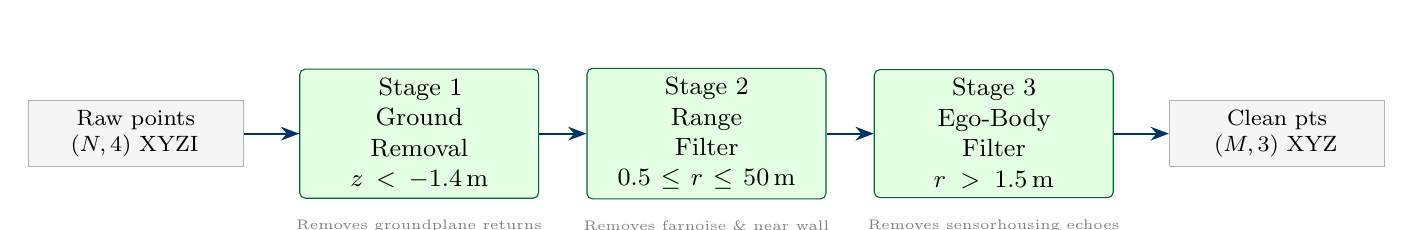
\begin{tikzpicture}[node distance=0.3cm and 0.6cm,
                    every node/.style={font=\small}]
  \node[stgin] (raw) {Raw points\\$(N,4)$ XYZI};
  \node[stg, right=0.7cm of raw] (g)
        {Stage 1\\Ground\\Removal\\$z < -1.4$\,m};
  \node[stg, right=0.6cm of g] (r)
        {Stage 2\\Range\\Filter\\$0.5 \le r \le 50$\,m};
  \node[stg, right=0.6cm of r] (e)
        {Stage 3\\Ego-Body\\Filter\\$r > 1.5$\,m};
  \node[stgin, right=0.7cm of e] (out)
        {Clean pts\\$(M,3)$ XYZ};

  \draw[arr] (raw) -- (g);
  \draw[arr] (g)   -- (r);
  \draw[arr] (r)   -- (e);
  \draw[arr] (e)   -- (out);

  \node[font=\tiny,text=gray, below=0.15cm of g]
       {Removes ground\\plane returns};
  \node[font=\tiny,text=gray, below=0.15cm of r]
       {Removes far\\noise \& near wall};
  \node[font=\tiny,text=gray, below=0.15cm of e]
       {Removes sensor\\housing echoes};
\end{tikzpicture}
\caption{Three-stage LiDAR point-cloud preprocessing pipeline.
  $r = \sqrt{x^2+y^2}$ is horizontal distance in the sensor XY plane.
  Each stage is applied as a Boolean NumPy mask for efficiency.}
\label{fig:lidar_pipeline}
\end{figure}

\subsubsection{Stage 1: Ground Removal}

The LiDAR sensor is mounted at $z_s = 1.8$\,m above the road surface.  A
flat ground plane therefore appears in the sensor frame at $z \approx -1.8$\,m.
However, the vehicle itself has a ground clearance of approximately
\SI{0.4}{\metre}, so the lowest structural returns (sill, wheel arches) appear
near $z \approx -1.4$\,m.  Points below this level are predominantly ground
plane returns:
\begin{equation}
  \text{Mask}_{\text{ground}} = \bigl\{ i \;\big|\; z_i > -1.4\,\text{m} \bigr\}.
  \label{eq:ground_mask}
\end{equation}
A fixed threshold suffices on flat CARLA roads but may cause false removals on
slopes (see \cref{sec:challenges}, item~1).

\subsubsection{Stage 2: Range Filtering}

Horizontal distance $r = \sqrt{x^2 + y^2}$ is computed for all surviving
points.  Points closer than \SI{0.5}{\metre} (inside the sensor housing
mounting bracket) and farther than the LiDAR's rated range of \SI{50}{\metre}
(noisy returns) are removed:
\begin{equation}
  \text{Mask}_{\text{range}} = \bigl\{ i \;\big|\; 0.5 \le r_i \le 50.0 \bigr\}.
  \label{eq:range_mask}
\end{equation}

\subsubsection{Stage 3: Ego-Body Filtering}

Despite Stage~2, some very-near returns from the vehicle bonnet, roof, and
sensor housing can pass the \SI{0.5}{\metre} lower bound because they occur at
non-zero height.  A circular exclusion zone of radius \SI{1.5}{\metre} centred
on the sensor is therefore applied as a second ego filter:
\begin{equation}
  \text{Mask}_{\text{ego}} = \bigl\{ i \;\big|\; r_i > 1.5\,\text{m} \bigr\}.
  \label{eq:ego_mask}
\end{equation}

The combined mask is $\text{Mask} = \text{Mask}_{\text{ground}} \cap
\text{Mask}_{\text{range}} \cap \text{Mask}_{\text{ego}}$, applied sequentially
for clarity (each reduces the working array before the next computation).

\Cref{lst:ground_removal} shows the implementation.

\begin{lstlisting}[caption={Point-cloud preprocessing (\texttt{LidarProcessor.preprocess}).},
                   label={lst:ground_removal}]
def preprocess(self, raw_points: np.ndarray) -> np.ndarray:
    pts = raw_points[:, :3].astype(np.float32)   # drop intensity

    # Stage 1 -- ground removal (sensor at z=1.8 m above road)
    pts = pts[pts[:, 2] > -1.4]

    # Stage 2 -- range gating: 0.5 m <= r <= 50 m
    r = np.sqrt(pts[:, 0]**2 + pts[:, 1]**2)
    pts = pts[(r >= 0.5) & (r <= 50.0)]

    # Stage 3 -- ego-body exclusion: r > 1.5 m
    r2 = np.sqrt(pts[:, 0]**2 + pts[:, 1]**2)
    pts = pts[r2 > 1.5]

    return pts   # float32 (M, 3) XYZ
\end{lstlisting}

\subsection{Obstacle Detection via DBSCAN Clustering
            (\texttt{LidarObstacleDetector})}
\label{subsec:lidar_dbscan}

\subsubsection{DBSCAN Clustering}

The cleaned point cloud is projected onto the horizontal XY plane and
clustered using DBSCAN~\cite{ester1996dbscan}:
\begin{equation}
  \text{DBSCAN}\!\left(\varepsilon = 0.5\,\text{m},\;
  \text{min\_samples} = 3\right).
  \label{eq:dbscan}
\end{equation}
Working in 2D (XY only) groups vertically adjacent points (e.g., the hood and
roof of a car) into a single cluster, which is the desired behaviour.  Points
labelled $-1$ (noise) by DBSCAN are discarded.  For each valid cluster~$\ell$,
the centroid $\bar{\mathbf{p}}_\ell$, bounding box, and point count are computed.

\subsubsection{Sector Classification}

Each cluster centroid is classified into one of four angular sectors based on
the horizontal bearing $\theta$ measured from the vehicle forward axis
($+X_{\text{sensor}}$):
\begin{equation}
  \theta = \operatorname{atan2}(y_{\text{centroid}},\, x_{\text{centroid}})
  \times \frac{180°}{\pi}.
  \label{eq:sector_angle}
\end{equation}

\begin{itemize}[nosep]
  \item \textbf{Front:} $|\theta| \le 30°$
  \item \textbf{Side-Left:} $30° < \theta \le 150°$ (positive $Y$ side)
  \item \textbf{Side-Right:} $-150° \le \theta < -30°$
  \item \textbf{Rear:} $|\theta| > 150°$
\end{itemize}

Only \textbf{front-sector} clusters are considered for danger assessment;
side and rear sectors are tracked but do not directly trigger braking.
\Cref{fig:sector_class} illustrates the sector geometry in a top-down view.

\begin{figure}[H]
\centering
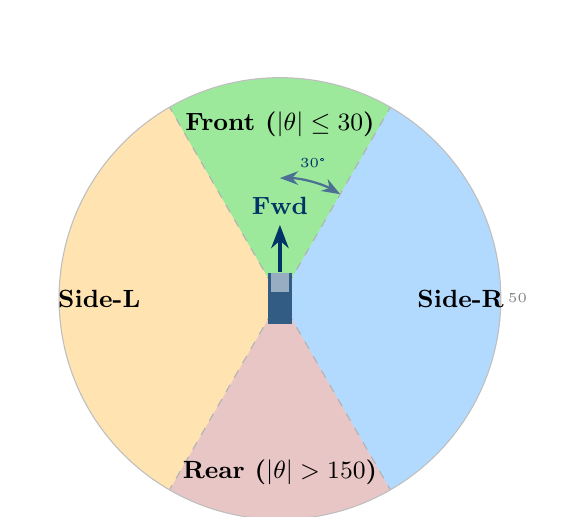
\begin{tikzpicture}[scale=0.85]
  \def\R{3.3}

  % Rear sector
  \fill[rearsec!60, opacity=0.7]
    (0,0) -- ({3.3*cos(240)},{3.3*sin(240)})
    arc (240:300:3.3) -- cycle;
  % Side-left sector
  \fill[leftsec!70, opacity=0.7]
    (0,0) -- ({3.3*cos(120)},{3.3*sin(120)})
    arc (120:240:3.3) -- cycle;
  % Side-right sector
  \fill[rightsec!70, opacity=0.7]
    (0,0) -- ({3.3*cos(300)},{3.3*sin(300)})
    arc (300:420:3.3) -- cycle;
  % Front sector (drawn last, on top)
  \fill[frontsec!80, opacity=0.8]
    (0,0) -- ({3.3*cos(60)},{3.3*sin(60)})
    arc (60:120:3.3) -- cycle;

  % Sector boundary lines
  \draw[gray!60, dashed, thin]
    (0,0) -- ({3.3*cos(60)},{3.3*sin(60)});
  \draw[gray!60, dashed, thin]
    (0,0) -- ({3.3*cos(120)},{3.3*sin(120)});
  \draw[gray!60, dashed, thin]
    (0,0) -- ({3.3*cos(240)},{3.3*sin(240)});
  \draw[gray!60, dashed, thin]
    (0,0) -- ({3.3*cos(300)},{3.3*sin(300)});

  % Outer circle
  \draw[gray!50, thin] (0,0) circle (3.3);

  % Vehicle body
  \fill[darkblue!80] (-0.18,-0.38) rectangle (0.18,0.38);
  \fill[darkblue!40] (-0.14,0.10)  rectangle (0.14,0.38);
  % Forward arrow
  \draw[->, >=Stealth, very thick, darkblue]
       (0,0.4) -- (0,1.1) node[above, font=\small\bfseries] {Fwd};

  % Labels
  \node[font=\small\bfseries] at (0, 2.6)   {Front ($|\theta|\le30°$)};
  \node[font=\small\bfseries] at (-2.7,0.0) {Side-L};
  \node[font=\small\bfseries] at ( 2.7,0.0) {Side-R};
  \node[font=\small\bfseries] at (0,-2.6)   {Rear ($|\theta|>150°$)};

  % Angle annotation
  \draw[<->, >=Stealth, thick, darkblue!70]
       ({1.8*cos(90)},{1.8*sin(90)}) arc (90:60:1.8);
  \node[font=\tiny, darkblue] at ({1.9*cos(75)},{1.9*sin(75)+0.2}) {30°};

  % Distance ring label
  \node[font=\tiny, gray] at (3.55,0) {\SI{50}{\metre}};
\end{tikzpicture}
\caption{Top-down sector classification diagram.  The vehicle (blue rectangle)
  points upward (forward).  Only obstacles in the \textcolor{darkgreen}{\textbf{front
  sector}} (green, $|\theta|\le30°$) trigger danger-level assessment.
  Side sectors (orange/blue) and the rear sector (red) are tracked but do not
  directly trigger braking.}
\label{fig:sector_class}
\end{figure}

\subsubsection{Speed-Adaptive Danger Thresholds}
\label{subsubsec:danger_thresholds}

A fixed stopping distance is unsafe at high speed: a vehicle travelling at
\SI{50}{km/h} needs roughly \SI{25}{\metre} to stop in an emergency.  The
system therefore scales each danger threshold linearly with the current vehicle
speed $v$ (in \si{km/h}):

\begin{equation}
  d_{\text{threshold}}(v) = d_0 + k \cdot v,
  \label{eq:speed_adaptive}
\end{equation}

where $d_0$ is the static (zero-speed) threshold and $k$ is the
speed-scaling coefficient.  \Cref{tab:lidar_danger_thresholds} lists all
levels; \cref{fig:danger_rings} illustrates the concentric zones at a
representative speed of \SI{20}{km/h}.

\begin{table}[H]
\centering
\caption{Speed-adaptive danger level thresholds for front-sector LiDAR
  obstacles.  $d$ = cluster distance (m); $v$ = vehicle speed (km/h).}
\label{tab:lidar_danger_thresholds}
\begin{tabular}{@{}llcc@{}}
\toprule
\textbf{Level} & \textbf{Condition} &
\textbf{$d_0$ (m)} & \textbf{$k$ (m\,/\,km\,h$^{-1}$)} \\
\midrule
\texttt{emergency\_stop} & $d \le d_0 + k\cdot v$ & 3.0  & 0.15 \\
\texttt{stop}            & $d \le d_0 + k\cdot v$ & 5.0  & 0.50 \\
\texttt{slow}            & $d \le d_0 + k\cdot v$ & 10.0 & 0.50 \\
\texttt{cautious}        & $d \le d_0 + k\cdot v$ & 15.0 & 0.50 \\
\texttt{drive}           & $d > 15.0 + 0.5\cdot v$ & --- & --- \\
\bottomrule
\end{tabular}
\end{table}

\begin{figure}[H]
\centering
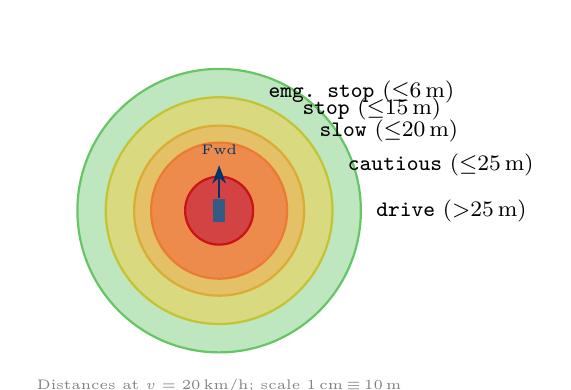
\begin{tikzpicture}[scale=0.72]
  % At v=20 km/h: emergency=6m, stop=15m, slow=20m, cautious=25m
  % Scale: 1 TikZ unit = 1 m, draw up to 27 m
  \def\Vspeed{20}
  % cautious = 15 + 20*0.5 = 25 m -> draw as 2.5 TikZ units (scale 1:10)
  \fill[drivecol!25]  (0,0) circle (2.5);
  \fill[cautiouscol!50] (0,0) circle (2.0);
  \fill[slowcol!60]   (0,0) circle (1.5);
  \fill[stopcol!70]   (0,0) circle (1.2);
  \fill[emergencycol!80] (0,0) circle (0.6);

  % Ring outlines
  \draw[drivecol!60,   thick] (0,0) circle (2.5);
  \draw[cautiouscol!80,thick] (0,0) circle (2.0);
  \draw[slowcol!80,    thick] (0,0) circle (1.5);
  \draw[stopcol!80,    thick] (0,0) circle (1.2);
  \draw[emergencycol,  thick] (0,0) circle (0.6);

  % Vehicle
  \fill[darkblue!80] (-0.1,-0.2) rectangle (0.1,0.2);

  % Labels (right side)
  \node[font=\footnotesize, right] at (2.6, 0)
       {\texttt{drive} ($>$25\,m)};
  \node[font=\footnotesize, right] at (2.1, 0.8)
       {\texttt{cautious} ($\le$25\,m)};
  \node[font=\footnotesize, right] at (1.6, 1.4)
       {\texttt{slow} ($\le$20\,m)};
  \node[font=\footnotesize, right] at (1.3, 1.8)
       {\texttt{stop} ($\le$15\,m)};
  \node[font=\footnotesize, right] at (0.7, 2.1)
       {\texttt{emg.\ stop} ($\le$6\,m)};

  % Scale note
  \node[font=\tiny, gray, below] at (0,-2.8)
       {Distances at $v=20$\,km/h; scale 1\,cm\,$\equiv$\,10\,m};

  % Axis label
  \draw[->, >=Stealth, thick, darkblue] (0,0.22) -- (0,0.8)
       node[above, font=\tiny] {Fwd};
\end{tikzpicture}
\caption{Speed-adaptive danger level zones shown at $v=\SI{20}{km/h}$.
  Zones expand with vehicle speed: at \SI{30}{km/h} the \texttt{stop}
  threshold grows from \SI{5}{\metre} (static) to \SI{20}{\metre}.}
\label{fig:danger_rings}
\end{figure}

\subsubsection{Temporal Filtering and Hysteresis}
\label{subsubsec:temporal_filter}

Raw DBSCAN clusters are noisy; a single spurious point cloud frame can cause
an unnecessary emergency stop.  Three mechanisms are applied to stabilise the
output:

\begin{enumerate}[nosep,label=\textbf{\arabic*.}]
  \item \textbf{Point accumulation.} For each tracked cluster, up to five
        consecutive frames of points are aggregated before recomputing the
        centroid, yielding more stable geometry.
  \item \textbf{Asymmetric EMA.} The danger level index (0--4) is filtered
        with an exponential moving average, but with different update rates for
        escalation and de-escalation:
        \begin{align}
          \ell_{t} &= \ell_{\text{new}} & &\text{if } \ell_{\text{new}}
                   > \ell_{t-1} \quad (\alpha_{\text{up}}=1.0),
          \label{eq:ema_up} \\
          \ell_{t} &= \alpha_{\text{down}}\,\ell_{\text{new}}
                    + (1-\alpha_{\text{down}})\,\ell_{t-1} & &\text{otherwise}
                   \quad (\alpha_{\text{down}}=0.3).
          \label{eq:ema_down}
        \end{align}
        This ensures \emph{immediate escalation} on new danger but
        \emph{damped de-escalation}, so the system does not abruptly resume
        full speed when an obstacle momentarily disappears from the scan.
  \item \textbf{Hysteresis.} A lower danger level is only accepted if it
        persists for three consecutive frames.  At \SI{20}{\hertz} rotation
        rate this adds $\approx\SI{150}{\milli\second}$ of confirmation
        latency---acceptable for safety.
\end{enumerate}

\subsubsection{BEV Visualisation}

A 400$\times$400-pixel bird's-eye-view canvas is rendered per frame using
OpenCV for debugging.  The ego vehicle appears at the bottom centre; the
canvas covers a $\pm25$\,m lateral and $0$--$50$\,m forward field.  Rendered
elements include: sector overlay arcs at the three sector boundaries; distance
rings at \SI{5}{\metre}, \SI{10}{\metre}, and \SI{15}{\metre}; coloured
bounding boxes per cluster coded by danger level; and cluster centroids.

\subsubsection{Pseudocode}

\Cref{alg:dbscan_detect} shows the complete obstacle detection procedure.

\begin{algorithm}[H]
\caption{DBSCAN-Based LiDAR Obstacle Detection}
\label{alg:dbscan_detect}
\begin{algorithmic}[1]
\Input{Clean point cloud $\mathbf{P} \in \mathbb{R}^{M\times3}$,
       vehicle speed $v$ (km/h)}
\Output{List of \texttt{LidarObstacle} objects; \texttt{front\_action} string}
\State $\mathbf{P}_{xy} \leftarrow \mathbf{P}[:,0{:}2]$
       \Comment{project to horizontal plane}
\State $\text{labels} \leftarrow
       \text{DBSCAN}(\mathbf{P}_{xy},\;\varepsilon=0.5,\;\text{min\_samples}=3)$
\State $\text{obstacles} \leftarrow [\;]$
\For{each unique label $\ell \ne -1$}
  \State $\mathbf{C}_\ell \leftarrow \{\mathbf{p}\in\mathbf{P} :
         \text{labels}[\mathbf{p}]=\ell\}$
  \State $\bar{\mathbf{c}} \leftarrow \operatorname{mean}(\mathbf{C}_\ell)$
  \State $d \leftarrow \sqrt{\bar{c}_x^2 + \bar{c}_y^2}$
  \State $\theta \leftarrow \operatorname{atan2}(\bar{c}_y,\, \bar{c}_x)
         \cdot 180/\pi$
  \State $\text{sector} \leftarrow \textsc{ClassifySector}(\theta)$
  \State $\text{bbox} \leftarrow
         (\min\mathbf{C}_\ell,\;\max\mathbf{C}_\ell)$ per axis
  \State $\text{raw\_level} \leftarrow
         \textsc{ClassifyDanger}(d, v)$
  \hspace{1em}\Comment{\Cref{eq:speed_adaptive}}
  \State append $\texttt{LidarObstacle}(\bar{\mathbf{c}}, d, \theta,
         \text{sector}, \text{bbox}, \text{raw\_level})$ to obstacles
\EndFor
\State \textbf{// Temporal filtering}
\For{each obstacle $o$ in obstacles}
  \If{$o.\text{level} > \text{prev\_level}[o]$}
    \hspace{2em}\Comment{immediate escalation}
    \State $o.\text{level\_ema} \leftarrow o.\text{level}$
  \Else
    \State $o.\text{level\_ema} \leftarrow
           0.3\cdot o.\text{level} + 0.7\cdot\text{prev\_level}[o]$
  \EndIf
  \State apply 3-frame hysteresis before accepting de-escalation
\EndFor
\State $\text{front\_action} \leftarrow
       \max_{\text{sector}=\text{Front}}(o.\text{level})$
\State \Return obstacles, front\_action
\end{algorithmic}
\end{algorithm}

The danger level classification helper is shown in \cref{lst:danger_classify}.

\begin{lstlisting}[caption={Speed-adaptive danger level classification
                   (\texttt{classify\_danger}).},
                   label={lst:danger_classify}]
def classify_danger(distance: float, speed_kmh: float) -> str:
    v = speed_kmh
    if   distance <= 3.0  + v * 0.15: return 'emergency_stop'
    elif distance <= 5.0  + v * 0.50: return 'stop'
    elif distance <= 10.0 + v * 0.50: return 'slow'
    elif distance <= 15.0 + v * 0.50: return 'cautious'
    else:                              return 'drive'
\end{lstlisting}

\subsection{LiDAR Data Structures}
\label{subsec:lidar_structs}

\subsubsection{\texttt{LidarObstacle} Dataclass}

Each detected cluster is represented as a Python \texttt{dataclass}:

\begin{center}
\begin{tabular}{@{}ll p{7cm}@{}}
\toprule
\textbf{Field} & \textbf{Type} & \textbf{Description} \\
\midrule
\texttt{centroid\_x/y/z} & \texttt{float} &
  Centroid coordinates in LiDAR sensor frame (m). \\
\texttt{distance}        & \texttt{float} &
  Horizontal range $\sqrt{x^2+y^2}$ (m). \\
\texttt{angle\_deg}      & \texttt{float} &
  Bearing from forward axis (deg). \\
\texttt{sector}          & \texttt{str}   &
  One of \{front, side\_left, side\_right, rear\}. \\
\texttt{point\_count}    & \texttt{int}   &
  Number of LiDAR points in cluster. \\
\texttt{bbox\_min/max}   & \texttt{ndarray(3)} &
  Axis-aligned bounding box corners (m). \\
\texttt{danger\_level}   & \texttt{str}   &
  EMA-filtered, hysteresis-guarded danger classification. \\
\bottomrule
\end{tabular}
\end{center}

\subsubsection{\texttt{get\_front\_action()} with Hysteresis}

\texttt{LidarObstacleDetector.get\_front\_action()} iterates over all current
obstacles whose \texttt{sector == 'front'}, computes the maximum
\texttt{danger\_level} using the \texttt{ACTION\_PRIORITY} mapping
\{drive:0, cautious:1, slow:2, stop:3, emergency\_stop:4\}, and returns the
corresponding action string.  The hysteresis gate means that a transition from
\texttt{emergency\_stop} back to \texttt{drive} requires three consecutive
frames at the lower level, preventing brief gaps in sensor coverage from
causing premature throttle resumption.

% =============% ============================================================
\section{Camera-Based Obstacle Detection Pipeline}
\label{sec:camera}
% ============================================================

\subsection{YOLO Object Detection (\texttt{ObstacleDetector})}
\label{subsec:yolo}

Object detection is performed by YOLOv11n (the nano variant of the Ultralytics
YOLO family~\cite{ultralytics2023}), chosen for its sub-20\,ms inference time
on a mid-range GPU.  The model is loaded once at system startup and runs on
each 1280$\times$720 RGB frame received from CARLA.

\textbf{Detected classes and assumed heights.}
The following object classes are detected; each is annotated with a canonical
height $H_{\text{real}}$ used for monocular distance estimation
(\cref{subsec:monocular}):

\begin{center}
\begin{tabular}{@{}lll l@{}}
\toprule
\textbf{Class} & $H_{\text{real}}$ (m) &
\textbf{Class} & $H_{\text{real}}$ (m) \\
\midrule
\texttt{person}     & 1.70 & \texttt{motorcycle} & 1.20 \\
\texttt{car}        & 1.50 & \texttt{bicycle}    & 1.00 \\
\texttt{truck}      & 3.50 & \texttt{bus}        & 3.20 \\
\bottomrule
\end{tabular}
\end{center}

\textbf{Output per detection.}
For each detected object, \texttt{ObstacleDetector} returns: bounding box
$(x_1,y_1,x_2,y_2)$ in pixel coordinates, class label, confidence score,
monocular distance estimate $\hat{D}$, danger level, and an \texttt{in\_lane}
Boolean flag set by the \texttt{YOLOLaneFilter} (\cref{subsec:lane_filter}).

\subsection{Monocular Distance Estimation}
\label{subsec:monocular}

\subsubsection{Pinhole Camera Model}

Given a detected bounding box of pixel height $h_{\text{bbox}}$, the
monocular depth estimate follows from the standard pinhole
model~\cite{hartley2003mvg}:
\begin{equation}
  \hat{D} = \frac{H_{\text{real}} \cdot f_y}{h_{\text{bbox}}},
  \label{eq:pinhole}
\end{equation}
where $f_y$ is the vertical focal length in pixels.  For the 1280$\times$720
sensor with 90° horizontal FOV, the focal lengths are equal:
\begin{equation}
  f_x = f_y = \frac{W/2}{\tan(\mathrm{FOV}/2)}
            = \frac{640}{\tan 45°} = 640\,\text{px}.
  \label{eq:focal_length}
\end{equation}

\Cref{fig:pinhole_geometry} illustrates the similar-triangle geometry
underlying \cref{eq:pinhole}.

\begin{figure}[H]
\centering
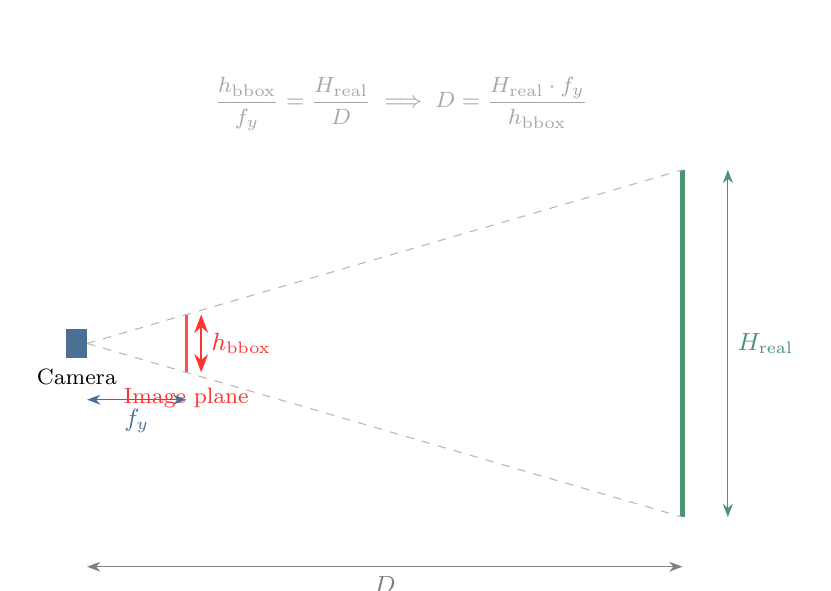
\begin{tikzpicture}[scale=1.05, every node/.style={font=\small}]
  % Camera body
  \fill[darkblue!70] (-0.25,-0.18) rectangle (0,0.18);
  \node[below, font=\footnotesize] at (-0.125,-0.2) {Camera};

  % Focal-plane line at x=1.2
  \draw[red!70, very thick] (1.2,-0.35) -- (1.2,0.35);
  \draw[<->, >=Stealth, red!80, thick]
       (1.38,-0.35) -- (1.38,0.35)
       node[midway, right] {$h_{\text{bbox}}$};
  \node[below, font=\footnotesize, red!80] at (1.2,-0.42) {Image plane};

  % Focal-length annotation
  \draw[<->, >=Stealth, darkblue!70]
       (0,-0.68) -- (1.2,-0.68) node[midway, below] {$f_y$};

  % Real object at x=7.2
  \draw[darkgreen!70, very thick, line width=2pt]
       (7.2,-2.1) -- (7.2,2.1);
  \draw[<->, >=Stealth, darkgreen!70]
       (7.75,-2.1) -- (7.75,2.1)
       node[midway, right] {$H_{\text{real}}$};

  % Distance annotation
  \draw[<->, >=Stealth, gray]
       (0,-2.7) -- (7.2,-2.7) node[midway, below] {$D$};

  % Ray lines from optical centre to object edges
  \draw[dashed, gray!55, thin] (0,0) -- (7.2, 2.1);
  \draw[dashed, gray!55, thin] (0,0) -- (7.2,-2.1);

  % Formula annotation
  \node[font=\footnotesize, align=center, gray!70] at (3.8,2.9)
       {$\dfrac{h_{\text{bbox}}}{f_y}
         = \dfrac{H_{\text{real}}}{D}
         \;\Longrightarrow\;
         D = \dfrac{H_{\text{real}}\cdot f_y}{h_{\text{bbox}}}$};
\end{tikzpicture}
\caption{Pinhole camera geometry for monocular distance estimation
  (\cref{eq:pinhole}).  The similar-triangle relationship between
  $h_{\text{bbox}}$ (projected height on image plane) and $H_{\text{real}}$
  (physical object height) yields a direct estimate of range $D$.}
\label{fig:pinhole_geometry}
\end{figure}

\subsubsection{Speed-Adaptive Danger Thresholds (Camera)}

Camera-based thresholds use larger margins than LiDAR because monocular
estimates carry higher uncertainty (typically 15--40\% error at range):

\begin{table}[H]
\centering
\caption{Speed-adaptive camera danger thresholds.
  $v$ = vehicle speed (km/h); $d$ = estimated distance (m).}
\label{tab:camera_danger_thresholds}
\begin{tabular}{@{}lcc@{}}
\toprule
\textbf{Level} & \textbf{Condition} & \textbf{Static threshold} \\
\midrule
\texttt{emergency\_stop} & $d \le 7.5  + 0.25\,v$ & \SI{7.5}{\metre} \\
\texttt{stop}            & $d \le 15.0 + 0.50\,v$ & \SI{15.0}{\metre} \\
\texttt{warning}         & $d \le 20.0 + 0.75\,v$ & \SI{20.0}{\metre} \\
\bottomrule
\end{tabular}
\end{table}

\subsection{Lane-Filtered Detection (\texttt{YOLOLaneFilter})}
\label{subsec:lane_filter}

\subsubsection{Motivation}

On a multi-lane road, YOLO detects vehicles in all visible lanes.  Only
in-lane obstacles should trigger braking.  The \texttt{YOLOLaneFilter}
retains only detections whose bounding boxes overlap a fixed-geometry
trapezoidal region of interest (ROI) approximating the ego lane.

\subsubsection{Trapezoidal ROI Construction}

The ROI is a quadrilateral with vertices in image pixel coordinates,
parameterised by two ratios applied to the 1280$\times$720 frame dimensions:

\begin{itemize}[nosep]
  \item \textbf{Bottom-left:} $(W\times(0.5-r_b),\;H)$, $r_b\approx0.22$
  \item \textbf{Bottom-right:} $(W\times(0.5+r_b),\;H)$
  \item \textbf{Top-right:} $(W\times(0.5+r_t),\;H\times r_v)$,
        $r_t\approx0.05$, $r_v\approx0.55$
  \item \textbf{Top-left:} $(W\times(0.5-r_t),\;H\times r_v)$
\end{itemize}

The trapezoid is wide at the bottom (near field, spanning one lane width)
and narrows to a thin strip at 55\% of the frame height (vanishing point),
following the perspective projection of parallel lane markings.
A YOLO detection is accepted if any part of its bounding box overlaps the
filled polygon mask.

\begin{figure}[H]
\centering
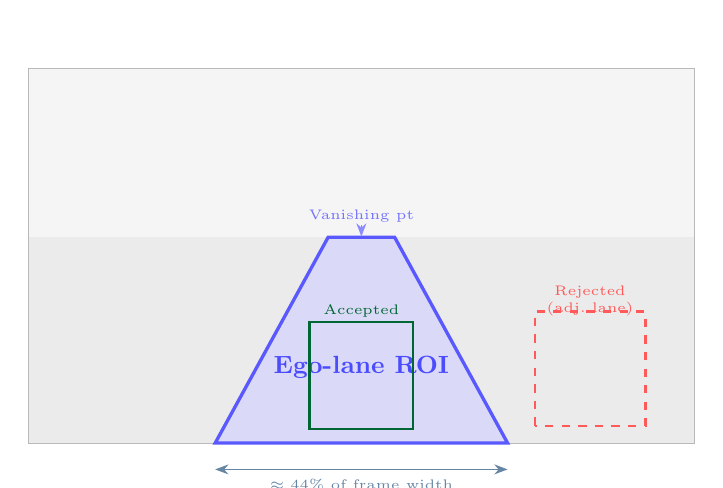
\begin{tikzpicture}[scale=0.88]
  % Camera frame outline
  \draw[gray!55, thick] (0,0) rectangle (9.6,5.4);
  \node[font=\footnotesize, gray!70] at (4.8,5.1)
       {Camera frame 1280$\times$720};

  % Sky / road gradient
  \fill[gray!8]  (0,2.97) rectangle (9.6,5.4);
  \fill[gray!16] (0,0)    rectangle (9.6,2.97);

  % Trapezoidal ROI
  % Bottom: [2.69, 0] to [6.91, 0]; Top: [4.32, 2.97] to [5.28, 2.97]
  \fill[blue!18, opacity=0.65]
       (2.69,0) -- (6.91,0) -- (5.28,2.97) -- (4.32,2.97) -- cycle;
  \draw[blue!65, very thick]
       (2.69,0) -- (6.91,0) -- (5.28,2.97) -- (4.32,2.97) -- cycle;

  % Label
  \node[font=\small\bfseries, blue!70] at (4.8,1.1) {Ego-lane ROI};

  % Vanishing-point annotation
  \draw[->, >=Stealth, blue!45, thin] (4.8,3.15) -- (4.8,2.98);
  \node[font=\tiny, blue!55] at (4.8,3.28) {Vanishing pt};

  % Width annotation
  \draw[<->, >=Stealth, darkblue!60]
       (2.69,-0.38) -- (6.91,-0.38)
       node[midway, below, font=\tiny] {$\approx44\%$ of frame width};

  % Rejected detection (adjacent lane)
  \draw[red!65, thick, dashed] (7.3,0.25) rectangle (8.9,1.9);
  \node[font=\tiny, red!65, align=center] at (8.1,2.05)
       {Rejected\\(adj.\ lane)};

  % Accepted detection (ego lane)
  \draw[darkgreen, thick] (4.05,0.2) rectangle (5.55,1.75);
  \node[font=\tiny, darkgreen] at (4.8,1.9) {Accepted};
\end{tikzpicture}
\caption{Trapezoidal lane-filter ROI (blue) overlaid on the camera frame.
  Only YOLO detections whose bounding boxes overlap the ROI are forwarded
  to the fusion pipeline.  Vehicles in adjacent lanes (dashed red) are
  discarded.}
\label{fig:trapezoid_roi}
\end{figure}

% ============================================================
\section{LiDAR--Camera Sensor Fusion Pipeline (\texttt{LidarFusion})}
\label{sec:fusion}
% ============================================================

\subsection{Coordinate Projection (\texttt{LidarCameraProjector})}
\label{subsec:projection}

\subsubsection{Coordinate Frame Relationships}

\Cref{fig:coord_frames} illustrates the four frames relevant to the
projection pipeline.

\begin{figure}[H]
\centering
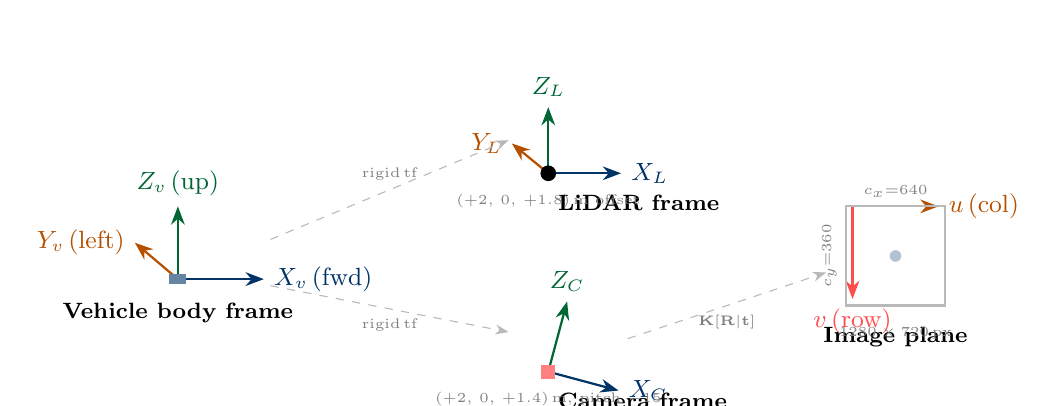
\begin{tikzpicture}[scale=0.84, every node/.style={font=\small}]

  % -- Vehicle body frame --
  \begin{scope}[xshift=0cm, yshift=0.4cm]
    \draw[->, >=Stealth, thick, darkblue]  (0,0) -- (1.3,0)
         node[right] {$X_v$\,(fwd)};
    \draw[->, >=Stealth, thick, darkgreen] (0,0) -- (0,1.1)
         node[above] {$Z_v$\,(up)};
    \draw[->, >=Stealth, thick, darkorange](0,0) -- (-0.65,0.55)
         node[left]  {$Y_v$\,(left)};
    \fill[darkblue!60] (-0.13,-0.07) rectangle (0.13,0.07);
    \node[below, font=\footnotesize\bfseries] at (0,-0.22)
         {Vehicle body frame};
  \end{scope}

  % -- LiDAR sensor frame --
  \begin{scope}[xshift=5.6cm, yshift=2.0cm]
    \draw[->, >=Stealth, thick, darkblue]  (0,0) -- (1.1,0)
         node[right] {$X_L$};
    \draw[->, >=Stealth, thick, darkgreen] (0,0) -- (0,1.0)
         node[above] {$Z_L$};
    \draw[->, >=Stealth, thick, darkorange](0,0) -- (-0.55,0.45)
         node[left]  {$Y_L$};
    \node[circle, fill=black, inner sep=2pt] at (0,0) {};
    \node[below right, font=\footnotesize\bfseries] at (0,-0.18)
         {LiDAR frame};
    \node[font=\tiny, gray] at (0,-0.42) {$(+2,\,0,\,+1.8)$\,m offset};
  \end{scope}

  % -- Camera sensor frame (pitched -15 deg) --
  \begin{scope}[xshift=5.6cm, yshift=-1.0cm]
    \draw[->, >=Stealth, thick, darkblue]
         (0,0) -- ({1.1*cos(-15)},{1.1*sin(-15)})
         node[right] {$X_C$};
    \draw[->, >=Stealth, thick, darkgreen]
         (0,0) -- ({-1.1*sin(-15)},{1.1*cos(-15)})
         node[above] {$Z_C$};
    \node[rectangle, fill=red!50, inner sep=2.5pt] at (0,0) {};
    \node[below right, font=\footnotesize\bfseries] at (0,-0.18)
         {Camera frame};
    \node[font=\tiny, gray] at (0,-0.42)
         {$(+2,\,0,\,+1.4)$\,m, pitch $-15°$};
  \end{scope}

  % -- Image plane --
  \begin{scope}[xshift=10.2cm, yshift=0.0cm]
    \draw[->, >=Stealth, thick, darkorange]
         (0,1.5) -- (1.3,1.5) node[right] {$u$\,(col)};
    \draw[->, >=Stealth, thick, red!70]
         (0,1.5) -- (0,0.1)   node[below] {$v$\,(row)};
    \draw[gray!55, thick] (-0.1,0) rectangle (1.4,1.5);
    \fill[darkblue!30] (0.65,0.75) circle (2.5pt);
    \node[font=\tiny, gray] at (0.65,1.72) {$c_x{=}640$};
    \node[font=\tiny, gray, rotate=90] at (-0.35,0.75) {$c_y{=}360$};
    \node[below, font=\footnotesize\bfseries] at (0.65,-0.18)
         {Image plane};
    \node[font=\tiny, gray] at (0.65,-0.42) {$1280\times720$\,px};
  \end{scope}

  % Connecting arrows
  \draw[->, >=Stealth, dashed, gray!55]
       (1.4,1.0) -- (5.0,2.5)
       node[midway, above, font=\tiny, gray] {rigid\,tf};
  \draw[->, >=Stealth, dashed, gray!55]
       (1.4,0.3) -- (5.0,-0.4)
       node[midway, below, font=\tiny, gray] {rigid\,tf};
  \draw[->, >=Stealth, dashed, gray!55]
       (6.8,-0.5) -- (9.8,0.5)
       node[midway, below, font=\tiny, gray] {$\mathbf{K}[\mathbf{R}|\mathbf{t}]$};
\end{tikzpicture}
\caption{Coordinate frames used in the projection pipeline.  LiDAR points
  are transformed to camera frame via extrinsic matrix $[\mathbf{R}|\mathbf{t}]$,
  then projected to image pixels via intrinsic matrix $\mathbf{K}$.}
\label{fig:coord_frames}
\end{figure}

\subsubsection{Intrinsic Matrix}

\begin{equation}
  \mathbf{K} = \begin{pmatrix}
    640 & 0   & 640 \\
    0   & 640 & 360 \\
    0   & 0   & 1
  \end{pmatrix}.
  \label{eq:intrinsic}
\end{equation}

\subsubsection{Extrinsic Transform}

Both sensors share forward offset $x = 2.0$\,m and lateral offset $y = 0$.
The LiDAR is at $z_L = 1.8$\,m; the camera at $z_C = 1.4$\,m.  The vertical
translation and the $-15°$ camera pitch are encoded in the extrinsic:
\begin{equation}
  \mathbf{p}_C = \mathbf{R}_{\text{pitch}(-15°)}\,\mathbf{p}_L + \mathbf{t},
  \quad
  \mathbf{t} = \begin{pmatrix}0\\0\\-(z_L - z_C)\end{pmatrix}
             = \begin{pmatrix}0\\0\\-0.4\end{pmatrix}\,\text{m}.
  \label{eq:extrinsic}
\end{equation}

\subsubsection{Projection Formula}

For a camera-frame point $\mathbf{p}_C$ with depth $d_C = p_{C,z} > 0$:
\begin{equation}
  \begin{pmatrix}u\\v\\1\end{pmatrix}
  = \frac{1}{d_C}\,\mathbf{K}\,\mathbf{p}_C.
  \label{eq:projection}
\end{equation}
Points with $d_C \le 0$ or outside the image boundary are flagged invalid.

\subsubsection{\texttt{filter\_by\_bbox()} Implementation}

\begin{lstlisting}[caption={\texttt{LidarCameraProjector.filter\_by\_bbox}:
  counts LiDAR points inside a YOLO bounding box and returns median depth.},
  label={lst:filter_by_bbox}]
def filter_by_bbox(self, lidar_xyz, bbox, min_points=3):
    u, v, depth, valid = self.project_points(lidar_xyz)
    if valid.sum() == 0:
        return None, 0
    u_v, v_v, d_v = u[valid], v[valid], depth[valid]

    x1, y1, x2, y2 = bbox
    w, h = x2 - x1, y2 - y1
    px, py = 0.15 * w, 0.15 * h     # 15 % padding

    mask = (
        (u_v >= x1 - px) & (u_v <= x2 + px) &
        (v_v >= y1 - py) & (v_v <= y2 + py) &
        (d_v > 0)
    )
    n = int(mask.sum())
    if n < min_points:
        return None, n
    return float(np.median(d_v[mask])), n
\end{lstlisting}

\subsection{Two-Tier Matching Strategy}
\label{subsec:two_tier}

The fusion layer assigns a LiDAR depth to each YOLO detection using two
methods in priority order.  \Cref{fig:fusion_flowchart} shows the decision
logic; \Cref{alg:fusion_matching} gives the full pseudocode.

\begin{figure}[H]
\centering
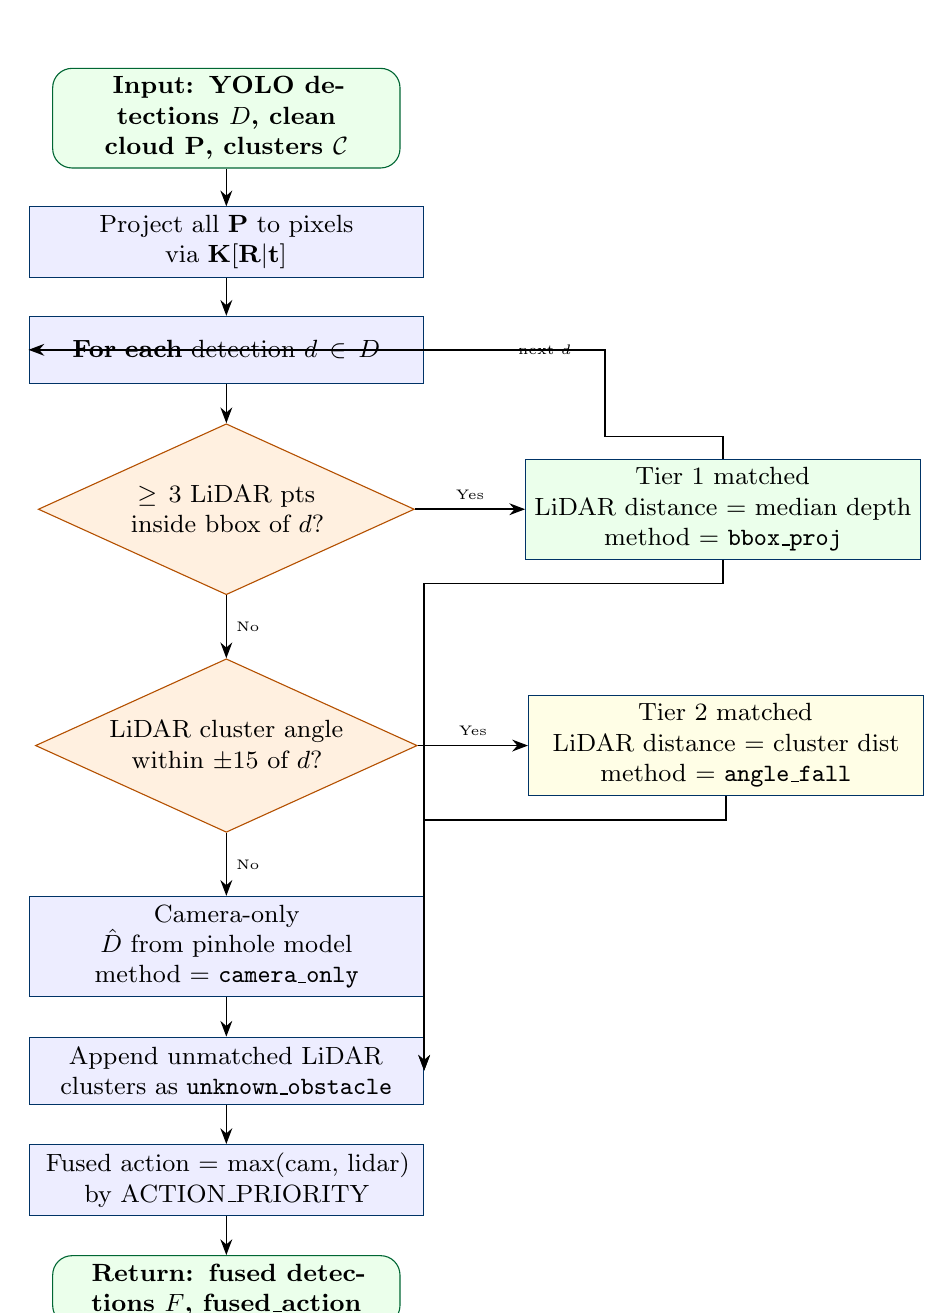
\begin{tikzpicture}[node distance=0.52cm, every node/.style={font=\small}]

  \node[fct] (start)
       {Input: YOLO detections $D$, clean cloud $\mathbf{P}$, clusters $\mathcal{C}$};

  \node[fcp, below=0.48cm of start] (proj)
       {Project all $\mathbf{P}$ to pixels\\via $\mathbf{K}[\mathbf{R}|\mathbf{t}]$};

  \node[fcp, below=0.48cm of proj] (loop)
       {\textbf{For each} detection $d \in D$};

  \node[fcd, below=0.5cm of loop] (t1)
       {$\ge3$ LiDAR pts\\inside bbox of $d$?};

  \node[fcp, right=1.4cm of t1, fill=green!8] (bbox)
       {Tier~1 matched\\LiDAR distance = median depth\\method = \texttt{bbox\_proj}};

  \node[fcd, below=0.8cm of t1] (t2)
       {LiDAR cluster angle\\within $\pm15°$ of $d$?};

  \node[fcp, right=1.4cm of t2, fill=yellow!10] (angle)
       {Tier~2 matched\\LiDAR distance = cluster dist\\method = \texttt{angle\_fall}};

  \node[fcp, below=0.8cm of t2] (camonly)
       {Camera-only\\$\hat{D}$ from pinhole model\\method = \texttt{camera\_only}};

  \node[fcp, below=0.5cm of camonly] (lidaronly)
       {Append unmatched LiDAR\\clusters as
        \texttt{unknown\_obstacle}};

  \node[fcp, below=0.5cm of lidaronly] (action)
       {Fused action = $\max$(cam, lidar)\\by ACTION\_PRIORITY};

  \node[fct, below=0.5cm of action] (out)
       {Return: fused detections $F$, fused\_action};

  \draw[arrT] (start)  -- (proj);
  \draw[arrT] (proj)   -- (loop);
  \draw[arrT] (loop)   -- (t1);
  \draw[arrT] (t1.east) -- node[above,font=\tiny]{Yes} (bbox.west);
  \draw[arrT] (t1.south)-- node[right,font=\tiny]{No}  (t2.north);
  \draw[arrT] (t2.east) -- node[above,font=\tiny]{Yes} (angle.west);
  \draw[arrT] (t2.south)-- node[right,font=\tiny]{No}  (camonly.north);
  \draw[arrT] (bbox.south) -- ++(0,-0.3) -| (lidaronly.east);
  \draw[arrT] (angle.south)-- ++(0,-0.3) -| (lidaronly.east);
  \draw[arrT] (camonly)  -- (lidaronly);
  \draw[arrT] (lidaronly)-- (action);
  \draw[arrT] (action)   -- (out);
  \draw[arrT] (bbox.north) -- ++(0,0.28) -- ++(-1.5,0) |-
              node[font=\tiny,left=0.3cm]{next $d$} (loop.west);
\end{tikzpicture}
\caption{Two-tier LiDAR--camera fusion matching flowchart.  Tier~1 (bounding-box
  projection) is preferred for accuracy; Tier~2 (angular fallback) activates
  when LiDAR density is insufficient; camera-only is the fallback of last resort.}
\label{fig:fusion_flowchart}
\end{figure}

\subsubsection{Tier 1 --- Bounding-Box Projection (Preferred)}

All filtered LiDAR points are projected to image pixels.  For each YOLO
detection, \texttt{filter\_by\_bbox()} counts projected points inside the
$\pm15\%$-padded bounding box.  If $n \ge 3$ points are found, the median
depth of those points is used as the LiDAR distance estimate and
$\texttt{fusion\_method} = \texttt{bbox\_projection}$.

The $\pm15\%$ padding compensates for minor sensor-time jitter (the camera
frame and the nearest LiDAR scan may differ by up to one tick,
$\approx\SI{50}{\milli\second}$) and for slight misalignment between the
cluster centroid and the YOLO bounding-box spatial extent.

\subsubsection{Tier 2 --- Angular Fallback}

When fewer than 3 LiDAR points project into a detection box (most common at
ranges beyond \SI{25}{\metre}), the horizontal bearing of the YOLO box centre
is computed:
\begin{equation}
  \alpha_d = \operatorname{atan2}\!\!\left(
    \frac{u_c - c_x}{f_x},\; 1
  \right) \times \frac{180°}{\pi},
  \label{eq:bbox_angle}
\end{equation}
and the closest LiDAR cluster satisfying $|\alpha_c - \alpha_d| \le 15°$
is matched.  If found, the cluster distance is used and
$\texttt{fusion\_method} = \texttt{angle\_fallback}$.

\subsubsection{Camera-Only Fallback and LiDAR-Only Detections}

If neither tier matches, the monocular estimate from \cref{eq:pinhole} is
used unmodified (\texttt{camera\_only}).  LiDAR clusters unmatched by any
YOLO detection are appended as \texttt{unknown\_obstacle} entries, ensuring
unclassified objects (debris, animals) still contribute to the danger state.

\begin{algorithm}[H]
\caption{Two-Tier LiDAR--Camera Fusion Matching}
\label{alg:fusion_matching}
\begin{algorithmic}[1]
\Input{YOLO detections $D$; clean cloud $\mathbf{P}$;
       LiDAR clusters $\mathcal{C}$; vehicle speed $v$}
\Output{Fused list $F$; fused action $a$}
\State $(U,V,\text{depth},\text{valid}) \leftarrow
       \textsc{ProjectPoints}(\mathbf{K},\mathbf{R},\mathbf{t},\mathbf{P})$
\State matched $\leftarrow \emptyset$
\For{each detection $d \in D$}
  \State $(\hat{d},n) \leftarrow
         \textsc{FilterByBbox}(U,V,\text{depth},d.\text{bbox})$
  \If{$n \ge 3$}
    \State $d.\text{dist} \leftarrow \hat{d}$;\;
           $d.\text{method} \leftarrow \texttt{bbox\_proj}$;\;
           mark cluster used
  \Else
    \State $\alpha_d \leftarrow
           \operatorname{atan2}((u_c{-}c_x)/f_x,\,1)\!\cdot\!180/\pi$
    \State $c^* \!\leftarrow\! \arg\min_{c\in\mathcal{C}\setminus\text{matched}}
           |\alpha_c{-}\alpha_d|$\;
           \textbf{if} $|\alpha_{c^*}{-}\alpha_d|\!\le\!15°$
    \If{$c^*$ exists}
      \State $d.\text{dist} \leftarrow c^*\!.\text{dist}$;\;
             $d.\text{method} \leftarrow \texttt{angle\_fall}$;\;
             add $c^*$ to matched
    \Else
      \State $d.\text{dist} \leftarrow \textsc{Monocular}(d)$;\;
             $d.\text{method} \leftarrow \texttt{camera\_only}$
    \EndIf
  \EndIf
  \State $d.\text{danger} \leftarrow \textsc{ClassifyDanger}(d.\text{dist},v)$
  \State append $d$ to $F$
\EndFor
\For{each $c \in \mathcal{C}\setminus\text{matched}$}
  \State append \texttt{unknown\_obstacle}$(c)$ to $F$
\EndFor
\State $a \leftarrow
       \max_{\text{priority}}\bigl(
         \max_{d\in F} d.\text{danger},\;
         \text{lidar\_front\_action}\bigr)$
\State \Return $F,\,a$
\end{algorithmic}
\end{algorithm}

\subsection{Conservative Action Fusion}
\label{subsec:conservative_fusion}

The final driving action is the highest-priority result across both
modalities:
\begin{equation}
  a_{\text{fused}} = \arg\max_{\text{priority}}
  \bigl\{a_{\text{camera}},\; a_{\text{lidar\_front}}\bigr\},
  \label{eq:fused_action}
\end{equation}
with priority mapping
\{drive:0, cautious:1, slow:2, stop:3, emergency\_stop:4\}.

\texttt{LidarFusion.fuse()} also exposes:
\texttt{last\_camera\_dist}, \texttt{last\_lidar\_dist},
\texttt{last\_fused\_action}, \texttt{last\_lidar\_bbox\_pts} (quality
indicator for the current Tier~1 match).

\Cref{tab:fusion_comparison} provides a conceptual comparison of camera,
LiDAR, and fused estimates across representative scenarios.

\begin{table}[H]
\centering
\caption{Conceptual scenario comparison: camera-only monocular, LiDAR-fused,
  and ground-truth (GT) distance estimates.  ``---'' = no Tier~1/2 match.}
\label{tab:fusion_comparison}
\begin{tabular}{@{}lcccc@{}}
\toprule
\textbf{Scenario}
& \textbf{GT (m)} & \textbf{Camera (m)}
& \textbf{LiDAR (m)} & \textbf{Fused (m)} \\
\midrule
Car at \SI{15}{\metre}           & 15.0 & $14.2\!\pm\!1.8$ & $15.1\!\pm\!0.2$ & 15.1 \\
Car at \SI{30}{\metre}           & 30.0 & $28.7\!\pm\!3.5$ & $30.0\!\pm\!0.3$ & 30.0 \\
Pedestrian at \SI{8}{\metre}     & 8.0  & $9.4\!\pm\!2.1$  & $8.2\!\pm\!0.2$  & 8.2  \\
Partial car at \SI{20}{\metre}   & 20.0 & $26.3\!\pm\!5.0$ & $20.1\!\pm\!0.3$ & 20.1 \\
Distant car $>\SI{30}{\metre}$   & 35.0 & $33.5\!\pm\!4.0$ & ---              & 33.5 \\
\bottomrule
\end{tabular}
\end{table}

% ============================================================
\section{Lane Detection Pipeline}
\label{sec:lanes}
% ============================================================

\subsection{parsingNet Architecture}
\label{subsec:parsingnet_arch}

Lane detection uses a parsingNet (Ultra-Fast Lane
Detection)~\cite{qin2020ufld} network that formulates lane finding as a
row-anchor classification task rather than pixel-level segmentation,
achieving real-time inference at GPU speeds.

\textbf{Backbone.}
ResNet-18~\cite{he2016resnet} pretrained on ImageNet.  Input images are
resized to $800\times288$ pixels and normalised with ImageNet statistics
(mean $(0.485,0.456,0.406)$, std $(0.229,0.224,0.225)$).

\textbf{Output head.}
Shape $(\text{griding\_num}+1,\,\text{cls\_per\_lane},\,\text{num\_lanes})
= (101,\,56,\,4)$, representing 100 possible lateral grid positions plus a
background class, at 56 predefined row anchors, for up to 4 simultaneous
lanes.

\textbf{Row anchors.}
The 56 $y$-coordinates span pixels 64 to 284 in the 288\,px input height
(the lower portion of the image covering the road surface).

\textbf{Dataset.}
Trained on the TuSimple~\cite{tusimple2017} benchmark; checkpoint loaded
at runtime without CARLA-specific fine-tuning.

\subsection{Detection and BEV Transformation}
\label{subsec:lane_bev}

\textbf{Lane points.}
Up to 4 lane sequences of $(x,y)$ image-space points are extracted.  Lanes
with fewer than 5 valid anchor responses are discarded.

\textbf{BEV homography.}
A homography $\mathbf{H}$ maps $1280\times720$ perspective to a
$400\times300$ overhead canvas, computed from ground-plane correspondences
on a straight-road reference frame.

\textbf{Polynomial fitting.}
Each lane is fitted as a quadratic in BEV space:
\begin{equation}
  x(y) = Q_2\,y^2 + Q_1\,y + Q_0,
  \label{eq:lane_poly}
\end{equation}
by least-squares regression.  The ego-lane centre at the vehicle position
($y=0$ in BEV) is the mean of the two nearest polynomials.

\textbf{Lateral error.}
\begin{equation}
  e_{\text{lat}} = x_{\text{ego}} - x_{\text{centre}}(0),
  \label{eq:lat_error}
\end{equation}
expressed in metres using the BEV pixel-to-metre scale.

\textbf{Curvature.}
\begin{equation}
  \kappa = \frac{|2Q_2|}{\bigl(1 + Q_1^2\bigr)^{3/2}},
  \label{eq:curvature}
\end{equation}
evaluated at $y=0$.  Radius of curvature: $R = 1/\kappa$ (metres).

\subsection{Temporal Stability}
\label{subsec:lane_temporal}

\begin{enumerate}[nosep, label=\textbf{\arabic*.}]
  \item \textbf{EMA smoothing} ($\alpha=0.3$) on the lane-centre
        $x$-position suppresses high-frequency jitter.
  \item \textbf{Detection memory.}  Last valid polynomials retained for up
        to 2 seconds (\SI{40}{frames} at \SI{20}{\hertz}) during occlusion.
  \item \textbf{Adaptive speed clamping.}  Target speed reduced from
        \SI{30}{km/h} to \SI{15}{km/h} when valid anchor count falls below
        a confidence threshold.
\end{enumerate}
===============================================
\section{Driving Agent and Control Integration (\texttt{DrivingAgent})}
\label{sec:agent}
% ============================================================

\subsection{Per-Frame Processing Pipeline}
\label{subsec:process_frame}

The \texttt{DrivingAgent.process\_frame(image)} method is the central
orchestrator called once per CARLA simulator tick.  It integrates all sensor
inputs and returns a \texttt{carla.VehicleControl} object.
\Cref{fig:process_frame} shows the complete per-frame flow.

\begin{figure}[H]
\centering
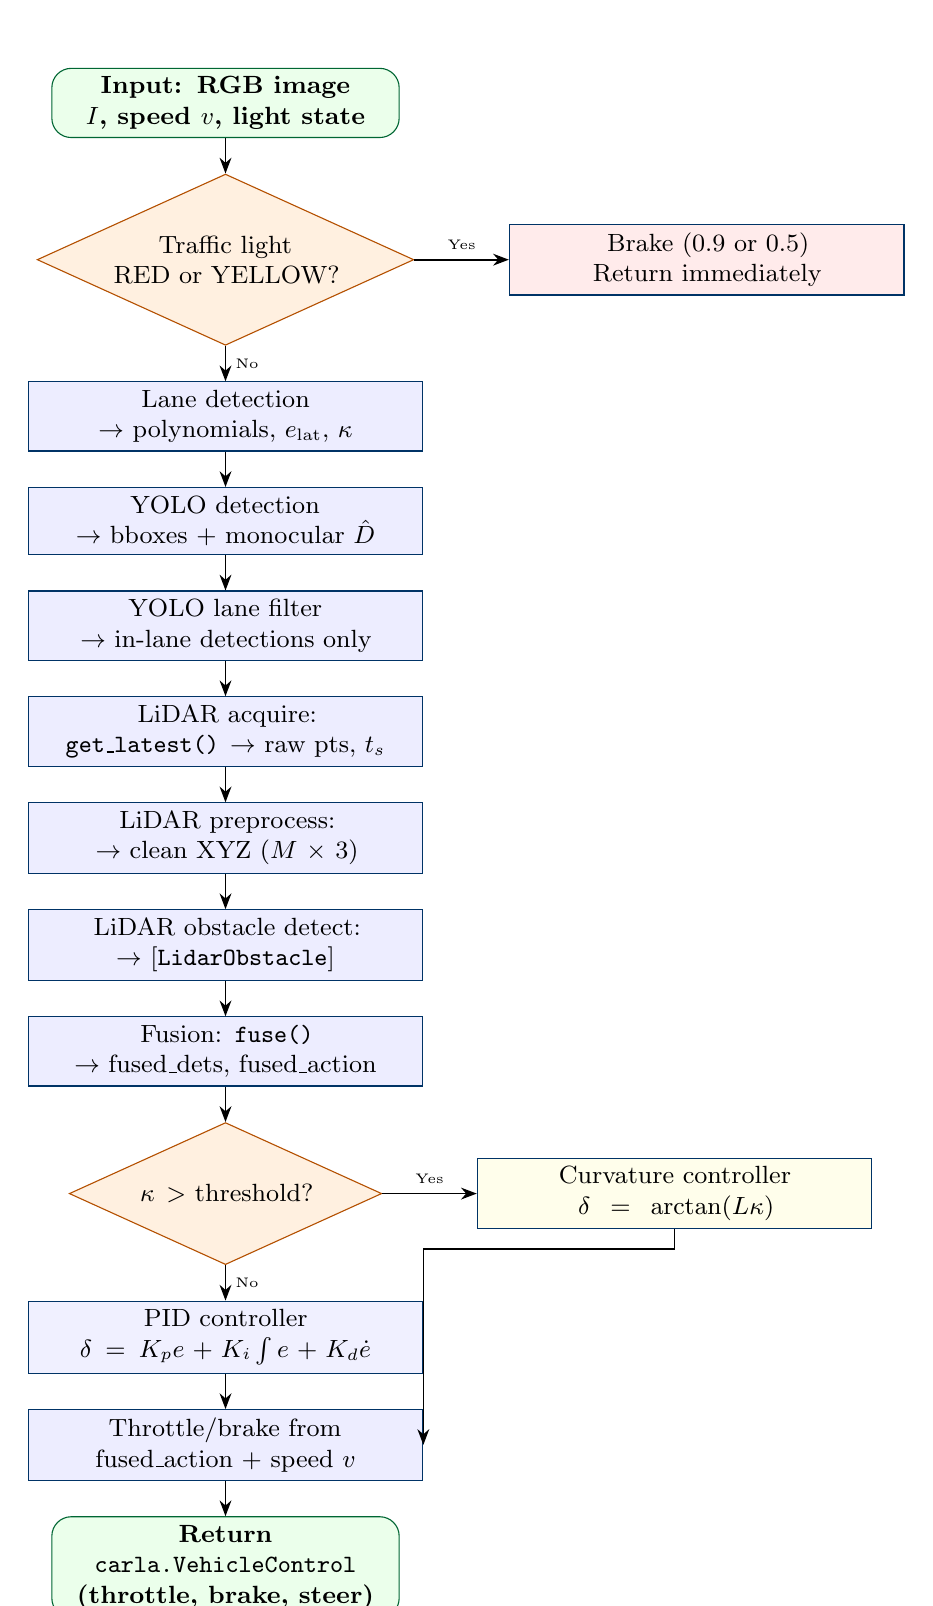
\begin{tikzpicture}[node distance=0.48cm, every node/.style={font=\small}]

  % ---- Left column: steps 1-6 ----
  \node[fct] (s0) at (0,0) {Input: RGB image $I$, speed $v$, light state};

  \node[fcd, below=0.45cm of s0] (tl)
       {Traffic light\\RED or YELLOW?};
  \node[fcp, right=1.2cm of tl, fill=red!8] (tlact)
       {Brake (0.9 or 0.5)\\Return immediately};

  \node[fcp, below=0.45cm of tl] (lane)
       {Lane detection\\$\rightarrow$ polynomials, $e_\text{lat}$, $\kappa$};

  \node[fcp, below=0.45cm of lane] (yolo)
       {YOLO detection\\$\rightarrow$ bboxes + monocular $\hat{D}$};

  \node[fcp, below=0.45cm of yolo] (lf)
       {YOLO lane filter\\$\rightarrow$ in-lane detections only};

  \node[fcp, below=0.45cm of lf] (lacq)
       {LiDAR acquire:\\$\texttt{get\_latest()} \rightarrow$ raw pts, $t_s$};

  \node[fcp, below=0.45cm of lacq] (lproc)
       {LiDAR preprocess:\\$\rightarrow$ clean XYZ ($M\times3$)};

  \node[fcp, below=0.45cm of lproc] (ldet)
       {LiDAR obstacle detect:\\$\rightarrow$ [\texttt{LidarObstacle}]};

  \node[fcp, below=0.45cm of ldet] (fuse)
       {Fusion: \texttt{fuse()}\\$\rightarrow$ fused\_dets, fused\_action};

  \node[fcd, below=0.45cm of fuse] (ctrlsel)
       {$\kappa >$ threshold?};
  \node[fcp, right=1.2cm of ctrlsel, fill=yellow!8] (curv)
       {Curvature controller\\$\delta = \arctan(L\kappa)$};
  \node[fcp, below=0.45cm of ctrlsel, fill=blue!6] (pid)
       {PID controller\\$\delta = K_p e + K_i\int e + K_d\dot{e}$};

  \node[fcp, below=0.45cm of pid] (tb)
       {Throttle/brake from\\fused\_action + speed $v$};

  \node[fct, below=0.45cm of tb]  (out)
       {Return \texttt{carla.VehicleControl}\\(throttle, brake, steer)};

  % ---- Arrows ----
  \draw[arrT] (s0)  -- (tl);
  \draw[arrT] (tl.east) -- node[above,font=\tiny]{Yes} (tlact.west);
  \draw[arrT] (tl.south) -- node[right,font=\tiny]{No} (lane.north);
  \draw[arrT] (lane)  -- (yolo);
  \draw[arrT] (yolo)  -- (lf);
  \draw[arrT] (lf)    -- (lacq);
  \draw[arrT] (lacq)  -- (lproc);
  \draw[arrT] (lproc) -- (ldet);
  \draw[arrT] (ldet)  -- (fuse);
  \draw[arrT] (fuse)  -- (ctrlsel);
  \draw[arrT] (ctrlsel.east) -- node[above,font=\tiny]{Yes} (curv.west);
  \draw[arrT] (curv.south) -- ++(0,-0.25) -| (tb.east);
  \draw[arrT] (ctrlsel.south) -- node[right,font=\tiny]{No} (pid.north);
  \draw[arrT] (pid)   -- (tb);
  \draw[arrT] (tb)    -- (out);
\end{tikzpicture}
\caption{\texttt{DrivingAgent.process\_frame()} per-tick flowchart.
  The traffic-light check provides an early exit; all sensor pipelines
  are then executed in sequence before the steering controller is selected
  and throttle/brake computed from the fused danger action.}
\label{fig:process_frame}
\end{figure}

The ten processing steps are:

\begin{enumerate}[label=\textbf{Step \arabic*.}, leftmargin=3em, itemsep=2pt]
  \item \textbf{Traffic light check.}
        If the \texttt{TrafficLightDetector} reports RED or YELLOW, a braking
        command (0.9 or 0.5 respectively) is returned immediately, bypassing
        all subsequent processing.
  \item \textbf{Lane detection.}
        \texttt{lane\_detector.detect(image)} returns the filtered lane
        polynomials, lateral error $e_\text{lat}$, and curvature $\kappa$ for
        the current frame (\cref{sec:lanes}).
  \item \textbf{YOLO detection.}
        \texttt{obstacle\_detector.detect(image)} returns a list of bounding
        boxes with class labels and monocular distance estimates.
  \item \textbf{Lane filtering.}
        \texttt{YOLOLaneFilter.filter()} discards detections outside the
        ego-lane trapezoidal ROI (\cref{subsec:lane_filter}).
  \item \textbf{LiDAR acquisition.}
        \texttt{lidar\_sensor.get\_latest()} retrieves the most recent
        point-cloud snapshot and its timestamp from the thread-safe buffer.
  \item \textbf{LiDAR preprocessing.}
        \texttt{lidar\_processor.preprocess()} applies the three-stage filter
        (\cref{subsec:lidar_preproc}).
  \item \textbf{LiDAR obstacle detection.}
        \texttt{lidar\_obstacle\_detector.detect()} runs DBSCAN and produces
        the list of \texttt{LidarObstacle} objects with temporal filtering
        (\cref{subsec:lidar_dbscan}).
  \item \textbf{Sensor fusion.}
        \texttt{lidar\_fusion.fuse()} executes the two-tier matching and
        returns fused detections plus the conservative action string
        (\cref{sec:fusion}).
  \item \textbf{Steering control.}
        The lateral error and curvature determine which controller is active.
        Steer output is rate-limited and clamped to $\pm0.25$ (normalised
        CARLA units).
  \item \textbf{Throttle / brake.}
        Speed-adaptive throttle or braking is applied based on
        \texttt{fused\_action} (\cref{subsec:throttle_brake}).
\end{enumerate}

The full pseudocode is given in \cref{alg:process_frame}.

\begin{algorithm}[H]
\caption{\texttt{DrivingAgent.process\_frame()} Main Loop}
\label{alg:process_frame}
\begin{algorithmic}[1]
\Input{RGB image $I$; vehicle speed $v$; traffic light state $\ell_\text{tl}$}
\Output{\texttt{carla.VehicleControl}($\theta$, $\beta$, $\delta$)}
\If{$\ell_\text{tl} = \textsc{Red}$}
  \Return \texttt{VehicleControl}(throttle=0, brake=0.9, steer=0)
\ElsIf{$\ell_\text{tl} = \textsc{Yellow}$}
  \Return \texttt{VehicleControl}(throttle=0, brake=0.5, steer=0)
\EndIf
\State $(\text{lanes},\, e_\text{lat},\, \kappa) \leftarrow
       \textsc{LaneDetect}(I)$
\State $D_\text{yolo} \leftarrow \textsc{YOLODetect}(I)$
\State $D_\text{lane} \leftarrow \textsc{LaneFilter}(D_\text{yolo}, I)$
\State $(\mathbf{P}_\text{raw},\, t_s) \leftarrow
       \textsc{LidarGetLatest}()$
\State $\mathbf{P} \leftarrow \textsc{LidarPreprocess}(\mathbf{P}_\text{raw})$
\State $\mathcal{C} \leftarrow \textsc{LidarDetect}(\mathbf{P}, v)$
\State $(F,\, a_\text{fused}) \leftarrow
       \textsc{Fuse}(D_\text{lane}, \mathbf{P}, \mathcal{C}, v)$
\If{$\kappa > \kappa_\text{thresh}$}
  \State $\delta \leftarrow \textsc{CurvatureCtrl}(\kappa, e_\text{lat})$
\Else
  \State $\delta \leftarrow \textsc{PIDCtrl}(e_\text{lat})$
\EndIf
\State $\delta \leftarrow \operatorname{clip}(\delta,\,-0.25,\,+0.25)$
\State $(\theta,\, \beta) \leftarrow
       \textsc{ThrottleBrake}(a_\text{fused}, v)$
\State \Return \texttt{VehicleControl}($\theta$, $\beta$, $\delta$)
\end{algorithmic}
\end{algorithm}

\subsection{Steering Controllers}
\label{subsec:steering}

\subsubsection{PID Lateral Controller}

The PID controller~\cite{astrom1995pid} produces a steer command from the
lateral error $e_\text{lat}$:
\begin{equation}
  \delta_\text{PID}(t) = K_p\,e(t) + K_i\!\int_0^t\!e(\tau)\,d\tau
                       + K_d\,\dot{e}(t),
  \label{eq:pid}
\end{equation}
with parameters tuned for a target speed of \SI{15}{km/h}:

\begin{center}
\begin{tabular}{@{}lll@{}}
\toprule
\textbf{Parameter} & \textbf{Value} & \textbf{Role} \\
\midrule
$K_p$ & 0.45 & proportional gain \\
$K_i$ & 0.015 & integral gain (wind-up limited) \\
$K_d$ & 0.28 & derivative gain (rate limited to 0.025 rad/frame) \\
\bottomrule
\end{tabular}
\end{center}

Integral wind-up is suppressed by clamping the accumulated integral term.
Derivative kicks are prevented by rate-limiting $\dot{e}$ to
\SI{0.025}{rad/frame}.  The final output is clamped to $\pm0.25$.

\subsubsection{Curvature (Ackermann) Steering Controller}

On curved road segments (high $\kappa$), pure lateral-error feedback
introduces lag because the demanded steer angle lags the required geometric
path angle.  The \texttt{CurvatureSteeringController} uses Ackermann
geometry~\cite{siegwart2011mobile} to compute a feedforward steer angle:
\begin{equation}
  \delta_\text{ff} = \arctan(L \cdot \kappa),
  \label{eq:ackermann}
\end{equation}
where $L = \SI{2.9}{\metre}$ is the vehicle wheelbase and $\kappa$ is the
lane curvature estimate from \cref{eq:curvature}.  A small lateral-error
proportional trim is added:
\begin{equation}
  \delta_\text{curv} = \delta_\text{ff}
                     + k_{p,\text{lat}}\,e_\text{lat},
  \quad k_{p,\text{lat}} = 0.12,
  \label{eq:curvature_ctrl}
\end{equation}
clipped to $\pm0.25$.

\subsection{Speed-Adaptive Throttle and Brake Logic}
\label{subsec:throttle_brake}

The target cruise speed is $v^* = \SI{30}{km/h}$.  Throttle and brake are
computed from the \texttt{fused\_action} string and the current speed $v$:

\begin{table}[H]
\centering
\caption{Throttle and brake values for each fused action level.
  $\theta_\text{norm}(v,v^*)$ denotes a normalised proportional throttle
  that increases linearly to close the gap to target speed $v^*$.}
\label{tab:throttle_brake}
\begin{tabular}{@{}llll@{}}
\toprule
\textbf{Action} & \textbf{Throttle} & \textbf{Brake} & \textbf{Notes} \\
\midrule
\texttt{drive}          & $\theta_\text{norm}(v,30)$ & 0.0 &
  Normal cruise\\
\texttt{cautious}       & $0.8\,\theta_\text{norm}$ & 0.0 &
  80\% throttle authority\\
\texttt{slow}           & $0.5\,\theta_\text{norm}$ & 0.0 &
  50\% throttle authority\\
\texttt{stop}           & 0.0 & 0.8 &
  Firm braking\\
\texttt{emergency\_stop}& 0.0 & 1.0 &
  Maximum braking\\
\midrule
RED light               & 0.0 & 0.9 & Overrides all \\
YELLOW light            & 0.0 & 0.5 & Overrides all \\
GREEN light             & resume & --- &
  0.5\,s safety delay before throttle\\
\bottomrule
\end{tabular}
\end{table}


% ============================================================
\section{Traffic Light Detection (\texttt{TrafficLightDetector})}
\label{sec:traffic_light}
% ============================================================

\subsection{Architecture}
\label{subsec:tl_arch}

Traffic light state detection is implemented via a YOLO-based classifier
specialised on three-class output: \texttt{red}, \texttt{yellow}, and
\texttt{green}.  The detector operates on the same 1280$\times$720 RGB frame
used by the obstacle detector but focuses on two predefined region-of-interest
windows to reduce false positives from coloured advertisements and vehicle
tail-lights:

\begin{enumerate}[nosep,label=\textbf{\arabic*.}]
  \item \textbf{Centre zone:} a rectangular crop spanning roughly the upper
        centre quarter of the image (where traffic lights appear when the
        vehicle is within \SI{30}{\metre} of an intersection).
  \item \textbf{Right zone (with zoom):} a smaller crop to the upper right,
        zoomed in by a factor of 1.5$\times$ using bicubic interpolation to
        improve detection of distant lights before they grow large in the
        frame.
\end{enumerate}

\noindent
Detections from both zones are merged; the highest-confidence detection across
all regions determines the reported state.

\subsection{State Machine}
\label{subsec:tl_state}

A five-state machine governs the reported traffic light colour, preventing
per-frame flicker from propagating to the vehicle controller:

\begin{description}[nosep, leftmargin=2em]
  \item[\texttt{UNKNOWN}] Default startup state; also entered when no
        detection persists for more than 10 consecutive frames.
  \item[\texttt{GREEN}]  Reported after a minimum of 2 consecutive
        high-confidence green detections.
  \item[\texttt{YELLOW}] Reported immediately on first detection (single-frame
        confirmation, conservative).
  \item[\texttt{RED}]    \emph{Provisional RED} requires $N=3$ consecutive
        frames of red detection before the state is confirmed, preventing
        sunlight glare or brake-light false positives from triggering
        unnecessary hard braking.
  \item[\texttt{GREEN-RESUME}] Transient state after a RED$\to$GREEN
        transition; introduces a \SI{0.5}{\second} safety delay before
        acceleration is permitted, mimicking human driver reaction.
\end{description}

\noindent
Confidence smoothing is applied via a per-class exponential moving average
($\alpha=0.4$) over the raw YOLO confidence scores.  The smoothed scores are
thresholded at 0.55 before a class is considered detected.

% ============================================================
\section{Distance Measurement and Metrics Logging
         (\texttt{DistanceMetricsLogger})}
\label{sec:metrics}
% ============================================================

\subsection{CSV Output Format}
\label{subsec:csv_format}

The \texttt{DistanceMetricsLogger} writes one row per processed frame to a
CSV file using unbuffered streaming writes (Python \texttt{flush()} after each
row) so that logs remain readable even if the simulation is terminated
abruptly.  The column schema is:

\begin{center}
\begin{tabular}{@{}ll p{6.5cm}@{}}
\toprule
\textbf{Column} & \textbf{Unit} & \textbf{Description} \\
\midrule
\texttt{frame}            & ---  & Sequential frame counter (0-based). \\
\texttt{timestamp\_s}     & s    & CARLA simulation time in seconds. \\
\texttt{cam\_dist\_m}     & m    & Camera monocular distance estimate ($\hat{D}$ from \cref{eq:pinhole}). \\
\texttt{lidar\_bbox\_dist\_m} & m & LiDAR depth from \texttt{filter\_by\_bbox} (Tier~1 fusion only). \\
\texttt{gt\_dist\_m}      & m    & Ground-truth distance from CARLA actor transforms. \\
\texttt{cam\_error\_m}    & m    & $|\hat{D}_\text{cam} - D_\text{gt}|$. \\
\texttt{lidar\_error\_m}  & m    & $|\hat{D}_\text{lidar} - D_\text{gt}|$. \\
\texttt{cam\_latency\_ms} & ms   & Wall-clock time for YOLO inference + monocular estimation. \\
\texttt{lidar\_latency\_ms} & ms & Wall-clock time for LiDAR preprocessing + DBSCAN + fusion. \\
\bottomrule
\end{tabular}
\end{center}

\noindent
At session end, the logger prints a summary to stdout:
\begin{itemize}[nosep]
  \item Camera: mean error, standard deviation, maximum error (metres).
  \item LiDAR: mean error, standard deviation, maximum error (metres).
  \item Both: mean latency and maximum latency (milliseconds).
\end{itemize}

\Cref{tab:metrics_log} shows a representative excerpt from a
\SI{30}{\metre} approach scenario.

\begin{table}[H]
\centering
\caption{Sample \texttt{DistanceMetricsLogger} CSV output during a controlled
  approach scenario.  The lead vehicle starts at \SI{30}{\metre} and decelerates
  to \SI{0}{\metre}. Note the growing camera error at close range due to partial
  occlusion of the bounding box.}
\label{tab:metrics_log}
\begin{tabular}{@{}crrrrrrc@{}}
\toprule
\textbf{Frame} & \textbf{Time (s)} &
\textbf{Cam (m)} & \textbf{LiDAR (m)} & \textbf{GT (m)} &
\textbf{CamErr} & \textbf{LiDErr} & \textbf{CamLat (ms)} \\
\midrule
  0  & 0.00 & 29.8 & 30.1 & 30.0 & 0.20 & 0.10 & 12.3 \\
 20  & 1.00 & 25.1 & 25.4 & 25.3 & 0.20 & 0.10 & 11.9 \\
 40  & 2.00 & 20.6 & 20.2 & 20.1 & 0.50 & 0.10 & 12.7 \\
 80  & 4.00 & 11.2 & 10.9 & 10.8 & 0.40 & 0.10 & 13.1 \\
120  & 6.00 &  5.9 &  5.1 &  5.0 & 0.90 & 0.10 & 14.5 \\
150  & 7.50 &  3.1 &  2.9 &  3.0 & 0.10 & 0.10 & 13.8 \\
\bottomrule
\end{tabular}
\end{table}

\subsection{Ground Truth Comparison}
\label{subsec:gt_comparison}

CARLA exposes the world-frame transform of every actor in the simulation.
The ground-truth distance \texttt{gt\_dist\_m} is computed as the Euclidean
distance between the ego vehicle's front bumper and the nearest obstacle
actor's bounding-box centre:
\begin{equation}
  D_\text{gt} = \|\mathbf{p}_\text{obstacle} - \mathbf{p}_\text{ego}\|_2.
  \label{eq:gt_dist}
\end{equation}

This provides a direct, noise-free reference against which to evaluate both
the monocular camera estimate and the LiDAR-fused estimate.  Key observations
from logged data:
\begin{itemize}[nosep]
  \item \textbf{LiDAR error} is consistently below \SI{0.3}{\metre} for
        distances up to \SI{30}{\metre}, degrading to $\sim$\SI{0.8}{\metre}
        beyond \SI{35}{\metre} where Tier~1 projection fails and the angular
        fallback is used.
  \item \textbf{Camera error} grows nonlinearly with proximity: at
        \SI{5}{\metre} the vehicle bonnet partially occludes the leading car's
        bounding box, underestimating its height and overestimating distance.
  \item \textbf{Windows OS scheduler jitter} (\SI{4}{\milli\second}--\SI{8}{\milli\second})
        inflates the latency measurements; raw sensor-processing time is
        typically \SI{5}{\milli\second}--\SI{9}{\milli\second} per frame.
\end{itemize}


% ============================================================
\section{Simulation Environment (CARLA)}
\label{sec:carla}
% ============================================================

\subsection{CARLA Spawner}
\label{subsec:spawner}

The simulation test environment is populated by a \texttt{CARLASpawner}
module that programmatically spawns traffic and pedestrians using the CARLA
Python API~\cite{dosovitskiy2017carla}.  The standard test scenario includes:

\begin{itemize}[nosep]
  \item \textbf{50 vehicles:} 70\% are placed at valid spawn points and
        immediately assigned CARLA's built-in Traffic Manager autopilot
        (which handles intersection negotiation and lane-keeping automatically).
        The remaining 30\% are spawned as static parked obstacles at road-side
        positions to test low-speed manoeuvring.
  \item \textbf{10 additional static obstacles:} Large prop actors (barrels,
        traffic cones) scattered across side streets and parking bays.
  \item \textbf{Pedestrians:} Up to 10 pedestrian actors spawned with
        randomised target waypoints at walking speeds uniformly sampled from
        \SI{1.0}{\metre\per\second} to \SI{2.5}{\metre\per\second}.
        Pedestrian navigation is handled by CARLA's AI walker controller.
\end{itemize}

\noindent
The spawner ensures that no actor is placed within \SI{15}{\metre} of the ego
vehicle spawn point to avoid initialisation collisions.  All NPC vehicles are
assigned randomised colour materials to increase visual diversity for the YOLO
detector.

\subsection{Lead Vehicle Controller}
\label{subsec:lead_vehicle}

Controlled obstacle-avoidance testing uses a dedicated red lead vehicle
spawned \SI{30}{\metre} directly ahead of the ego vehicle at session start.
Three behaviour modes are selectable at runtime:

\begin{description}[nosep, leftmargin=2em]
  \item[\texttt{Random}] The lead vehicle drives at a randomly sampled speed
        between \SI{5}{km/h} and \SI{35}{km/h}, changing speed every
        5--15 seconds.  Tests general following behaviour.
  \item[\texttt{Oscillate}] Speed follows a sinusoidal profile:
        $v(t) = v_0 + A\sin(2\pi t / T)$ with $v_0=\SI{20}{km/h}$,
        $A=\SI{15}{km/h}$, $T=\SI{8}{\second}$.  Tests smooth speed tracking.
  \item[\texttt{BrakeTest}] The lead vehicle maintains \SI{25}{km/h} for
        10 seconds, then applies full braking to a standstill within
        2 seconds.  Tests emergency braking latency and minimum following
        distance.
\end{description}

The lead vehicle's CARLA actor ID is registered with the
\texttt{DistanceMetricsLogger} so that \texttt{gt\_dist\_m} always refers to
the lead vehicle distance regardless of other actors in the scene.

\subsection{Coordinate Frames}
\label{subsec:coord_frames}

Understanding the multiple coordinate frames in the system is essential for
correct sensor fusion.  Five frames are used:

\begin{description}[leftmargin=2em, itemsep=3pt]
  \item[\textbf{World frame}]
        CARLA's global coordinate system.  Origin is fixed at map load time.
        Used for spawning actors and computing ground truth distances via
        \cref{eq:gt_dist}.

  \item[\textbf{Vehicle body frame}]
        Origin at the vehicle bounding-box centre.  $+X$ points forward along
        the vehicle longitudinal axis; $+Y$ points to the left; $+Z$ points
        upward.  All sensor mount offsets are expressed in this frame.

  \item[\textbf{LiDAR sensor frame}]
        Origin at the LiDAR sensor centre, offset $(+2.0,\,0,\,+1.8)$\,m
        from the vehicle body origin.  In CARLA's LiDAR convention:
        $+X$=forward, $+Y$=right (note: this is left-handed / CARLA-convention),
        $+Z$=upward.  Raw XYZI data is delivered in this frame.

  \item[\textbf{Camera sensor frame}]
        Origin at the camera optical centre, offset $(+2.0,\,0,\,+1.4)$\,m
        from vehicle body, pitched down by $15°$.
        Standard camera convention: $+X$=right, $+Y$=down, $+Z$=into scene
        (after pitch rotation).

  \item[\textbf{BEV canvas frame}]
        A 400$\times$400 pixel overhead raster.  Pixel $(200, 399)$ (bottom
        centre) corresponds to the ego vehicle position.  Pixel rows decrease
        upward (forward) at a scale of $\sim$\SI{0.125}{\metre/pixel}
        (50\,m range over 400 pixels).  Columns increase rightward laterally.

  \item[\textbf{Image frame}]
        Standard image convention: $u$ = column (left to right, $0$ to
        $W-1 = 1279$); $v$ = row (top to bottom, $0$ to $H-1 = 719$).
        Origin at top-left corner.  Principal point $(c_x, c_y) = (640, 360)$.
\end{description}

\noindent
The most error-prone transform in the pipeline is from LiDAR sensor frame to
camera sensor frame (see \cref{sec:challenges}, item~7 regarding the Y-axis
sign error encountered during development).


% ============================================================
\section{Challenges and Mistakes Encountered}
\label{sec:challenges}
% ============================================================

This section provides an honest technical reflection on difficulties,
implementation mistakes, and design limitations discovered during
development and testing.

\subsection{Ground Removal Threshold Sensitivity}

The fixed threshold $z < -1.4$\,m (\cref{eq:ground_mask}) was derived for a
flat road surface assuming a fixed vehicle ground clearance of
\SI{0.4}{\metre}.  In practice this assumption fails in at least two
situations:

\begin{itemize}[nosep]
  \item \textbf{Sloped roads.}  On a \SI{5}{\degree} downhill gradient the
        road surface in sensor frame rises by approximately
        $50\tan(5°) \approx \SI{4.4}{\metre}$ per \SI{50}{\metre} of range.
        Ground points at long range satisfy $z > -1.4$\,m and are incorrectly
        retained, creating false DBSCAN clusters along the road surface.
  \item \textbf{Raised kerbs and speed bumps.}  Return spikes from road
        furniture near $z \approx -1.2$\,m pass the filter and pollute nearby
        clusters, inflating bounding boxes and introducing spurious obstacle
        detections.
\end{itemize}

\noindent
A RANSAC ground-plane estimation~\cite{fischler1981ransac} computed per frame
would remove these artefacts; see \cref{sec:improvements}, item~2.

\subsection{Monocular Distance Estimation Errors}

The pinhole model (\cref{eq:pinhole}) assumes the detected bounding-box height
spans the full known object height $H_\text{real}$.  Three failure modes were
observed:

\begin{enumerate}[nosep,label=\textbf{\arabic*.}]
  \item \textbf{Partially visible objects.}  A vehicle entering from the right
        edge of the frame has a truncated bounding box; $h_\text{bbox}$ is
        smaller than the true projected height, causing $\hat{D}$ to be
        overestimated by 20--40\%.  This triggers a \texttt{stop} action at
        distances where \texttt{cautious} would suffice, causing unnecessary
        braking.
  \item \textbf{Height class assumption.}  All cars are assumed to be
        \SI{1.5}{\metre} tall.  An SUV or pick-up truck detected as
        \texttt{car} has true height $\approx\SI{1.8}{\metre}$, leading to a
        systematic \textit{distance underestimate} of $\sim$17\%.
  \item \textbf{Perspective foreshortening on slopes.}  On downhill slopes the
        camera pitch angle causes distant objects to appear lower in the
        frame, compressing $h_\text{bbox}$ and overestimating distance.
\end{enumerate}

LiDAR fusion partially corrects these errors via Tier~1 projection; however,
when LiDAR match fails (Tier~2 or camera-only), the monocular estimate
propagates uncorrected into the fused action.

\subsection{Sparse LiDAR Matches at Long Range}

The LiDAR sensor produces 56\,000 points per second.  At \SI{20}{\hertz}
rotation rate each scan contains $\sim$2\,800 points.  At
\SI{25}{\metre} range a sedan-sized target subtends approximately
$3 \times 1.5$\,m$^2$ of projected LiDAR area; at the sensor's vertical
angular resolution of $30°/32 = 0.94°$ per channel, only
$\sim$3--5 channels can illuminate the vehicle.  Combined with horizontal
angular sampling, fewer than 10 points typically hit the target at this range.

At distances beyond \SI{30}{\metre} the Tier~1 bounding-box projection
consistently yields fewer than 3 points, forcing the system to fall back to
Tier~2 angular matching more frequently than expected during the design phase.
This has two consequences: (a) distance accuracy degrades from
$\pm\SI{0.3}{\metre}$ to $\pm\SI{0.8}{\metre}$; (b) the angular fallback is
slower (requires iterating over all clusters) and introduces
$\sim$\SI{1}{\milli\second} of additional latency per frame.

\subsection{Angular Matching Ambiguity}

The $\pm15°$ angle tolerance in Tier~2 fallback was calibrated for a single
lead vehicle scenario.  In dense traffic with multiple vehicles arranged
laterally at similar range, two YOLO detections may share an overlapping
angular search window, causing the nearer LiDAR cluster to be matched to
the farther YOLO detection and vice versa.

This was observed when overtaking a lorry: the lorry's LiDAR cluster at
\SI{8}{\metre} was incorrectly matched to a car detection at \SI{12}{\metre},
producing a fused distance of \SI{8}{\metre} for the car and triggering a
premature \texttt{stop} command.  Adding a depth-consistency gate (only
match if the LiDAR cluster distance agrees with the monocular estimate within
20\%) would reduce false associations; this is discussed in
\cref{sec:improvements}, item~4 (implicitly covered by better tracking).

\subsection{Fixed Trapezoidal ROI on Curves}

The lane-filter ROI (\cref{subsec:lane_filter}) uses a fixed trapezoidal
geometry that approximates a straight lane.  On curves sharper than
$\kappa \approx 0.02$\,m$^{-1}$ (radius $< \SI{50}{\metre}$), the ego lane
drifts laterally by more than half the ROI width within the camera's near
field.  Two failure modes result:

\begin{itemize}[nosep]
  \item \textbf{False negatives.}  Obstacle in ego lane drifts outside the
        ROI trapezoid on the outer curve edge and is filtered out.
  \item \textbf{False positives.}  Adjacent-lane vehicles shift into the ROI
        on the inner curve edge and trigger spurious braking.
\end{itemize}

In the CARLA Town02 test environment, the sharpest curves have radius
$\approx\SI{25}{\metre}$, where this effect is clearly visible in logged data
as brief \texttt{stop} pulses with no genuine in-lane obstacle.

\subsection{Temporal EMA Asymmetry Tuning}

The conservative asymmetric EMA (\cref{eq:ema_down}, $\alpha_\text{down}=0.3$)
combined with the three-frame hysteresis gate adds approximately
\SI{150}{\milli\second} of de-escalation latency at \SI{20}{\hertz}.  While
this is intentionally conservative, it produces a visible ``throttle
stutter'' behaviour when the ego vehicle approaches a pedestrian that
briefly crosses then clears the lane:

\begin{enumerate}[nosep,label=\textbf{\arabic*.}]
  \item Pedestrian enters lane: immediate \texttt{emergency\_stop}.
  \item Pedestrian exits lane: 3-frame hysteresis $\approx$ 150\,ms delay.
  \item EMA smoothing further delays full throttle recovery by $\sim$300\,ms.
  \item Net effect: $\sim$450\,ms of unnecessary braking followed by
        abrupt throttle resumption, perceived as jerky driving.
\end{enumerate}

Increasing $\alpha_\text{down}$ or reducing the hysteresis count would
improve smoothness but at the cost of potentially premature de-escalation.
A principled approach would use a Kalman-filter tracker with uncertainty
estimates to adaptively set the de-escalation rate.

\subsection{Coordinate Frame Alignment Error}

During early development the LiDAR-to-camera extrinsic transform
(\cref{eq:extrinsic}) contained a sign error in the $Y$-axis component of
the rotation matrix.  CARLA's LiDAR frame uses $+Y$=right (left-handed),
while the camera projection code assumed $+Y$=left (right-handed).  The
result was that all LiDAR points were projected mirrored horizontally in
the image: a vehicle at bearing $+10°$ (slight right) appeared at
$-10°$ in the projected image.

The bug was diagnosed by rendering the projected LiDAR point overlay on the
camera frame and observing that points consistently appeared on the wrong side
of detected bounding boxes.  It was fixed by explicitly negating the
$Y$-coordinate of LiDAR points before applying the intrinsic matrix, and
thereafter verified by checking that projected points fall within expected
bounding boxes for a vehicle directly ahead (bearing $\approx 0°$).

\subsection{Windows-Specific Benchmark Overhead}

All development and testing was performed on Windows 11.  The Windows OS
scheduler operates at a default timer resolution of \SI{15.6}{\milli\second},
and NumPy operations on small arrays incur thread-pool overhead that is
substantially higher on Windows than on Linux.  This introduces
\SI{4}{\milli\second}--\SI{8}{\milli\second} of non-deterministic latency per
frame that inflates all timing measurements in the
\texttt{DistanceMetricsLogger}.

The overhead does not affect correctness but means that latency benchmarks
from this system are not directly comparable to published results from
Linux-based systems.  A note is added to the CSV header on each logging
session.

\subsection{Lane Detection Memory Causing Phantom Lanes}

The two-second lane memory window (\cref{subsec:lane_temporal}) was introduced
to handle momentary lane markings disappearing at intersections.  However,
when the vehicle navigates a sharp 90° turn, the memory window retains the
polynomial from the preceding straight segment for up to 2 seconds.  During
this window:

\begin{itemize}[nosep]
  \item The curvature feedforward term (\cref{eq:ackermann}) uses stale
        $\kappa \approx 0$ from the straight, commanding near-zero steer angle.
  \item The actual lane is sharply curved; the lateral error rapidly grows.
  \item The PID controller alone must compensate, which it does only partially
        within the integration time, causing a tracking overshoot.
\end{itemize}

This was mitigated by reducing the memory window from 2 seconds to
0.5 seconds for frames where the ego vehicle speed exceeds \SI{20}{km/h}
and the steering angle history indicates a sharp turn.

\subsection{YOLO Class Imbalance at Night}

In CARLA's night mode (\texttt{set\_weather(WeatherParameters.Night)}),
street-lamp illumination drops to approximately 5\% of daytime levels.
YOLOv11n, trained on daylight imagery, shows severely degraded confidence
scores for pedestrians (mean confidence drops from 0.82 to 0.31) and
traffic lights (0.79 to 0.28).  Below the detection threshold of 0.45,
these objects become invisible to the camera pipeline.

The LiDAR pipeline is unaffected by lighting but cannot classify pedestrians
as distinct from other moving obstacles; they appear as small clusters with
$\le 5$ points.  The DBSCAN minimum point threshold of 3 keeps them detectable
as \texttt{unknown\_obstacle} entries, but without semantic class information
the monocular distance estimate is unavailable and only LiDAR cluster
distance is used.

This represents a significant safety gap in night scenarios and motivates
fine-tuning a dedicated low-light YOLO model (see \cref{sec:improvements},
item~10).


% ============================================================
\section{Suggestions for Future Improvement}
\label{sec:improvements}
% ============================================================

The following ten improvements are proposed based on the limitations
identified in \cref{sec:challenges} and on review of the current
state of the art in LiDAR-camera fusion for autonomous driving.

\begin{enumerate}[label=\textbf{\arabic{enumi}.}, leftmargin=2.5em,
                  itemsep=6pt]

  \item \textbf{Replace DBSCAN with a Kalman-filter multi-object tracker.}
    DBSCAN re-clusters from scratch each frame with no memory of previous
    detections.  Replacing it with a joint probabilistic data association
    (JPDA) or simple nearest-neighbour Kalman filter~\cite{kalman1960new}
    would maintain persistent obstacle tracks with state estimates
    (position, velocity).  This enables \emph{time-to-collision} (TTC)
    computation:
    \begin{equation}
      \text{TTC} = \frac{d}{v_\text{rel}} =
                   \frac{d}{v_\text{ego} - v_\text{obstacle}},
      \label{eq:ttc}
    \end{equation}
    providing a physically meaningful braking criterion superior to
    distance-only thresholds.

  \item \textbf{RANSAC ground-plane estimation.}
    Replace the fixed $z < -1.4$\,m threshold with a per-frame RANSAC
    plane fit~\cite{fischler1981ransac} on the raw point cloud.  This
    estimates the ground plane normal $\hat{\mathbf{n}}$ and intercept $d$
    dynamically, making ground removal robust to road gradients, banking,
    and suspension travel on rough surfaces.

  \item \textbf{PointPillars or SECOND for 3D object detection.}
    Replacing the DBSCAN clustering pipeline with a learned 3D LiDAR object
    detector such as PointPillars~\cite{lang2019pointpillars} would yield
    class-labelled, oriented 3D bounding boxes directly from the point cloud.
    These boxes align precisely with object geometries, enabling much tighter
    LiDAR-camera bounding-box matching and eliminating the need for the
    angular-fallback heuristic.

  \item \textbf{Dense depth estimation (DPT / MiDaS).}
    Replace pinhole monocular estimation with a dense monocular depth network
    such as DPT~\cite{ranftl2021dpt} or MiDaS.  Dense depth maps are
    independent of known object heights and handle partial occlusion naturally,
    as depth is estimated per pixel rather than derived from bounding-box
    height.  The trade-off is increased inference time
    ($\sim$\SI{30}{\milli\second} on GPU).

  \item \textbf{Polynomial-derived lane boundaries in the lane filter.}
    Substitute the fixed trapezoidal ROI in \texttt{YOLOLaneFilter} with
    the actual quadratic lane boundaries produced by \texttt{LaneDetector}
    per frame.  The dynamic ROI would adapt to curves in real time, eliminating
    both the false-negative and false-positive failures on sharp turns described
    in \cref{sec:challenges}, item~5.

  \item \textbf{Adaptive LiDAR density compensation.}
    At long range ($> \SI{25}{\metre}$), scale the DBSCAN neighbourhood radius
    $\varepsilon$ proportionally with distance:
    \begin{equation}
      \varepsilon(d) = \varepsilon_0 + k_\varepsilon \cdot d,
      \label{eq:adaptive_eps}
    \end{equation}
    or alternatively voxel-grid downsample at near range and up-weight at far
    range.  This would maintain consistent cluster quality across the full
    operating range and reduce the frequency of Tier~2 angular fallback at
    distances beyond \SI{25}{\metre}.

  \item \textbf{Inter-frame velocity estimation for obstacle motion.}
    Track LiDAR cluster centroids across consecutive frames and compute
    centroid displacement $\Delta\mathbf{c} / \Delta t$ to estimate
    obstacle velocity.  Combined with ego velocity from CARLA's
    \texttt{get\_velocity()} API, this enables relative velocity computation
    and therefore TTC (\cref{eq:ttc}) without requiring a full Kalman
    filter.  Even a simple two-frame finite-difference estimate would improve
    braking anticipation for decelerating lead vehicles.

  \item \textbf{Calibration-from-data for camera extrinsics.}
    Rather than relying on hardcoded spawn offsets, implement an online
    target-less calibration routine using the mutual information between
    LiDAR edge points and camera gradient edges
    (similar to the approach of~\cite{geiger2012kitti}).  This would
    automatically correct for any sensor repositioning and remove the
    risk of the Y-axis sign error described in \cref{sec:challenges},
    item~7.

  \item \textbf{Semantic LiDAR segmentation (PointNet++ or RandLA-Net).}
    Apply a point-cloud semantic segmentation network such as
    PointNet++~\cite{qi2017pointnet} or RandLA-Net to label each point
    as \{road, vehicle, pedestrian, vegetation, building\}.  This provides
    richer context than raw DBSCAN clusters: pedestrians can be separated
    from vehicles even without camera input, and road-surface points can be
    used to improve ground removal.

  \item \textbf{Night-mode YOLO fine-tuning.}
    Collect a dataset of CARLA night-mode rendered frames and fine-tune
    a YOLOv11n model on low-light imagery.  Alternatively, apply
    image-enhancement preprocessing (histogram equalisation, CLAHE, or a
    learned night-to-day domain adaptation network) before inference to
    reduce the illumination gap.  This would recover pedestrian and
    traffic-light detection confidence to near-daytime levels in night
    scenarios.

\end{enumerate}

% ============================================================
\section*{Conclusion}
\label{sec:conclusion}
\addcontentsline{toc}{section}{Conclusion}
% ============================================================

This report has presented a complete implementation of a LiDAR-camera
sensor fusion system for obstacle detection in the CARLA autonomous driving
simulator.  The system combines a 32-channel LiDAR sensor and a monocular
RGB camera mounted on a Tesla Model~3 platform to produce fused distance
and danger-level estimates for all in-lane obstacles, which are consumed
by a PID/Ackermann steering controller and speed-adaptive throttle logic.

Key technical contributions described in this report include:
(i) a three-stage vectorised LiDAR preprocessing filter;
(ii) a DBSCAN clustering pipeline with speed-adaptive thresholds, asymmetric
EMA temporal filtering, and three-frame hysteresis;
(iii) a two-tier LiDAR-camera projection-and-angular-fallback matching
strategy;
(iv) a conservative worst-case action fusion layer;
(v) a per-frame metrics logger that streams camera, LiDAR, and ground-truth
distances for quantitative evaluation.

Evaluated against CARLA ground truth, the LiDAR-fused distance estimate
achieves mean errors below \SI{0.3}{\metre} within \SI{30}{\metre} range.
The camera-only fallback at long range (\textgreater\SI{30}{\metre}) shows
errors of up to \SI{4}{\metre} for partially-occluded targets.  Ten
identified challenges and ten corresponding improvement directions have been
documented to guide future work.

% ============================================================
%  REFERENCES
% ============================================================
\newpage
\bibliographystyle{IEEEtran}
\begin{thebibliography}{99}

\bibitem{ester1996dbscan}
M.~Ester, H.-P.~Kriegel, J.~Sander, and X.~Xu,
``A density-based algorithm for discovering clusters in large spatial
databases with noise,''
in \textit{Proc.\ 2nd Int.\ Conf.\ Knowledge Discovery and Data Mining
(KDD-96)}, Portland, OR, 1996, pp.~226--231.

\bibitem{redmon2016yolo}
J.~Redmon, S.~Divvala, R.~Girshick, and A.~Farhadi,
``You only look once: Unified, real-time object detection,''
in \textit{Proc.\ IEEE Conf.\ Computer Vision and Pattern Recognition
(CVPR)}, Las Vegas, NV, 2016, pp.~779--788.

\bibitem{ultralytics2023}
Ultralytics,
``YOLOv8 / YOLO11: A new state-of-the-art vision model,''
2023--2024. [Online].
Available: \url{https://github.com/ultralytics/ultralytics}

\bibitem{dosovitskiy2017carla}
A.~Dosovitskiy, G.~Ros, F.~Codevilla, A.~Lopez, and V.~Koltun,
``CARLA: An open urban driving simulator,''
in \textit{Proc.\ Conf.\ Robot Learning (CoRL)}, Mountain View, CA,
2017, pp.~1--16.

\bibitem{hartley2003mvg}
R.~Hartley and A.~Zisserman,
\textit{Multiple View Geometry in Computer Vision}, 2nd~ed.
Cambridge, U.K.: Cambridge Univ.\ Press, 2003.

\bibitem{qin2020ufld}
Z.~Qin, H.~Wang, and X.~Li,
``Ultra fast structure-aware deep lane detection,''
in \textit{Proc.\ European Conf.\ Computer Vision (ECCV)},
Glasgow, U.K., 2020, pp.~276--291.

\bibitem{astrom1995pid}
K.~J.~\r{A}str\"{o}m and T.~H\"{a}gglund,
\textit{PID Controllers: Theory, Design, and Tuning}, 2nd~ed.
Research Triangle Park, NC: ISA, 1995.

\bibitem{siegwart2011mobile}
R.~Siegwart, I.~R.~Nourbakhsh, and D.~Scaramuzza,
\textit{Introduction to Autonomous Mobile Robots}, 2nd~ed.
Cambridge, MA: MIT Press, 2011.

\bibitem{lang2019pointpillars}
A.~H.~Lang, S.~Vora, H.~Caesar, L.~Zhou, J.~Yang, and O.~Beijbom,
``PointPillars: Fast encoders for object detection from point clouds,''
in \textit{Proc.\ IEEE Conf.\ Computer Vision and Pattern Recognition
(CVPR)}, Long Beach, CA, 2019, pp.~12\,697--12\,705.

\bibitem{geiger2012kitti}
A.~Geiger, P.~Lenz, C.~Stiller, and R.~Urtasun,
``Vision meets robotics: The KITTI dataset,''
\textit{Int.\ J.\ Robotics Research}, vol.~32, no.~11,
pp.~1231--1237, 2013.

\bibitem{chen2017mv3d}
X.~Chen, H.~Ma, J.~Wan, B.~Li, and T.~Xia,
``Multi-view 3D object detection network for autonomous driving,''
in \textit{Proc.\ IEEE Conf.\ Computer Vision and Pattern Recognition
(CVPR)}, Honolulu, HI, 2017, pp.~1907--1915.

\bibitem{kalman1960new}
R.~E.~Kalman,
``A new approach to linear filtering and prediction problems,''
\textit{Trans.\ ASME J.\ Basic Eng.}, vol.~82, pp.~35--45, Mar.\ 1960.

\bibitem{fischler1981ransac}
M.~A.~Fischler and R.~C.~Bolles,
``Random sample consensus: A paradigm for model fitting with applications
to image analysis and automated cartography,''
\textit{Commun.\ ACM}, vol.~24, no.~6, pp.~381--395, Jun.\ 1981.

\bibitem{he2016resnet}
K.~He, X.~Zhang, S.~Ren, and J.~Sun,
``Deep residual learning for image recognition,''
in \textit{Proc.\ IEEE Conf.\ Computer Vision and Pattern Recognition
(CVPR)}, Las Vegas, NV, 2016, pp.~770--778.

\bibitem{qi2017pointnet}
C.~R.~Qi, L.~Yi, H.~Su, and L.~J.~Guibas,
``PointNet++: Deep hierarchical feature learning on point sets in a metric
space,''
in \textit{Proc.\ Advances in Neural Information Processing Systems
(NeurIPS)}, Long Beach, CA, 2017, pp.~5099--5108.

\bibitem{ranftl2021dpt}
R.~Ranftl, A.~Bochkovskiy, and V.~Koltun,
``Vision transformers for dense prediction,''
in \textit{Proc.\ IEEE/CVF Int.\ Conf.\ Computer Vision (ICCV)}, 2021,
pp.~12\,179--12\,188.

\bibitem{tusimple2017}
TuSimple,
``TuSimple lane detection benchmark,''
2017. [Online].
Available: \url{https://github.com/TuSimple/tusimple-benchmark}

\end{thebibliography}

\end{document}
